%%%%%%%%%%%%%%%%%%%%%%%%%%%%%%%%%%%%%%%%%%%%%%%
%
% Template per Elaborato di Laurea
% DISI - Dipartimento di Ingegneria e Scienza dell’Informazione
%
% update 2015-09-10
%
% Per la generazione corretta del 
% pdflatex nome_file.tex
% bibtex nome_file.aux
% pdflatex nome_file.tex
% pdflatex nome_file.tex
%
%%%%%%%%%%%%%%%%%%%%%%%%%%%%%%%%%%%%%%%%%%%%%%%

% formato FRONTE RETRO
\documentclass[epsfig,a4paper,11pt,titlepage,twoside,openany]{book}
\usepackage{epsfig}
\usepackage{plain}
\usepackage{setspace}
\usepackage[paperheight=29.7cm,paperwidth=21cm,outer=1.5cm,inner=2.5cm,top=2cm,bottom=2cm]{geometry} % per definizione layout
\usepackage{titlesec} % per formato custom dei titoli dei capitoli

\usepackage[utf8x]{inputenc} 

\singlespacing

\usepackage[british]{babel}

%% My packages
\usepackage{silence}\WarningsOff[latexfont]
\usepackage{amsmath}
\usepackage{amsfonts}
\usepackage{amssymb}
\usepackage{graphicx}
\graphicspath{images/}
\usepackage{cite}
\usepackage{url}
\usepackage{subcaption}
\usepackage{float}
\usepackage[ruled,vlined,linesnumbered]{algorithm2e}
\SetKwProg{Fn}{Event}{}{}
\SetKw{And}{and}
\usepackage[binary-units,per-mode=symbol]{siunitx}
\sisetup{list-final-separator = {, and },detect-weight=true, detect-family=true}
\usepackage{booktabs}
\usepackage{pifont}
\usepackage{microtype}
\usepackage{textcomp}
\usepackage[capitalise]{cleveref}
\def\figname{\csname cref@figure@name\endcsname\xspace}
\def\tabname{\csname cref@table@name\endcsname\xspace}
\def\secname{\csname cref@section@name\endcsname\xspace}
\def\eqpname{\csname cref@equation@name@plural\endcsname\xspace}
\crefname{algorithm}{Listing}{Lists.}
\Crefname{algorithm}{Listing}{Listings}
\SetAlgorithmName{Listing}{Listing}{List of Listings}
\crefname{lstlisting}{listing}{listings}
\Crefname{lstlisting}{Listing}{Listings}
\usepackage{xspace}
\usepackage{hyphenat}
\usepackage[draft,inline,nomargin,index]{fixme}
\fxsetup{theme=color}
\usepackage{grffile}
\usepackage{xfrac}
\usepackage{multirow}
\usepackage[font={small}]{caption}
\usepackage{imakeidx}

\usepackage{tikz}
\usetikzlibrary{calc,shapes,arrows,fit,positioning}

%listings configuration
\usepackage{listings}
\lstset{
   language=sh,
   columns=fixed,
   breaklines=true,
   breakatwhitespace=true,
   prebreak=\textbackslash,
   basicstyle=\ttfamily\small,
   showstringspaces=false,
   upquote=true,
   keywordstyle=\ttfamily\small
}

\usepackage{color}
\definecolor{gray}{rgb}{0.4,0.4,0.4}
\definecolor{darkblue}{rgb}{0.0,0.0,0.6}
\definecolor{cyan}{rgb}{0.0,0.6,0.6}

\lstdefinelanguage{XML}
{
  morestring=[b]",
  morestring=[s]{>}{<},
  morecomment=[s]{<?}{?>},
  stringstyle=\color{black},
  identifierstyle=\color{darkblue},
  keywordstyle=\color{cyan},
  morekeywords={xmlns,version,type}% list your attributes here
}

\definecolor{codegreen}{rgb}{0,0.6,0}
\definecolor{codegray}{rgb}{0.5,0.5,0.5}
\definecolor{codepurple}{rgb}{0.58,0,0.82}
\definecolor{backcolour}{rgb}{0.95,0.95,0.92}

\lstdefinestyle{shell}{
    backgroundcolor=\color{backcolour},
    breakatwhitespace=false,
    breaklines=true,
    captionpos=b,
    keepspaces=true,
    showspaces=false,
    showstringspaces=false,
    showtabs=false,
    tabsize=2
}

\lstdefinestyle{graphml}{
    backgroundcolor=\color{backcolour},
    breakatwhitespace=false,
    breaklines=true,
    captionpos=b,
    keepspaces=true,
    showspaces=false,
    showstringspaces=false,
    showtabs=false,
    tabsize=2
}

\lstMakeShortInline[language=bash]|

% fix cleveref and breqn
\makeatletter
\let\cref@old@eq@setnumberOld\eq@setnumber
\def\eq@setnumber{%
\cref@old@eq@setnumberOld%
\cref@constructprefix{equation}{\cref@result}%
\protected@xdef\cref@currentlabel{%
[equation][\arabic{equation}][\cref@result]\p@equation\eq@number}}
\makeatother

\RequirePackage{xstring}
\RequirePackage{xparse}
\RequirePackage[index=true]{acro}
\NewDocumentCommand\acrodef{mO{#1}mG{}}{\DeclareAcronym{#1}{short={#2}, long={#3}, #4}}
\NewDocumentCommand\acused{m}{\acuse{#1}}

% Acronim definition
\acrodef{ADV}{advertisement}
\acrodef{AS}{Autonomous System}{short-plural=es}
\acrodef{BGP}{Border Gateway Protocol}
\acrodef{BIRD}{BGP Internet Routing Daemon}
\acrodef{DPC}{Destination Partial Centrality}
\acrodef{eBGP}{Exterior BGP}
\acrodef{ERP}{Exterior Routing Protocol}
\acrodef{IP}{Internet Protocol}
\acrodef{MRAI}{Minimum Route Advertisement Interval}
\acrodef{NH}{Next Hop}
\acrodef{RFC}{Request For Comment} 
\acrodef{TCP}{Transmission Control Protocol}
\acrodef{FSM}{Finite State Machine}
\acrodef{DES}{Descrete Event Simulator}
\acrodef{RFD}{Route Flap Damping}
\acrodef{RNG}{Random Number Generator}

\newcommand{\figwidthfour}{0.78}
\newcommand{\figwidth}{0.78}
\newcommand{\figvspace}{-1.5em}

\begin{document}

  % nessuna numerazione
  \pagenumbering{gobble} 
  \pagestyle{plain}

\thispagestyle{empty}

\begin{center}
  \begin{figure}[h!]
    \centerline{
\psfig{file=images/marchio_unitrento_colore_it_202002.eps,width=0.6\textwidth}}
  \end{figure}

  \vspace{2 cm} 

  \LARGE{Dept. of Information Engineering and Computer Science\\}

  \vspace{1 cm} 
  \Large{Master's Degree in\\
	Computer Science
  }

  \vspace{2 cm} 
  \Large\textsc{Final Dissertation\\} 
  \vspace{1 cm} 
  \Huge\textsc{BGP, Catch the noise\\}
  \Large{\it{A study on the noise detectors of BGP and their correlation}}


  \vspace{2 cm} 
  \begin{tabular*}{\textwidth}{ c @{\extracolsep{\fill}} c }
  \Large{Supervisors} & \Large{graduating student}\\
  \Large{Renato Antonio Lo Cigno\\Timothy G Griffin}& \Large{Milani Mattia}\\
  \end{tabular*}

  \vspace{2 cm} 

  \Large{Accademic Year 2019/2020}
  
  \vspace{2 cm} 

  \Large{In collaboration with the University of Cambridge}
  
\end{center}



  \clearpage
 
  \thispagestyle{empty}

\begin{center}
  {\bf \Huge Thanks}
\end{center}

\vspace{4cm}


\emph{
  Thanks to everyone who believed in me
}

  \clearpage
  \pagestyle{plain} % nessuna intestazione e pie pagina con numero al centro

  % inizio numerazione pagine in numeri arabi
  \mainmatter

  % indice
  \tableofcontents
  \clearpage
  
  % gruppo per definizone di successione capitoli senza interruzione di pagina
  \begingroup
    % redefinizione del formato del titolo del capitolo
    % da formato
    %   Capitolo X
    %   Titolo capitolo
    % a formato
    %   X   Titolo capitolo
    
    \titleformat{\chapter}
      {\normalfont\Huge\bfseries}{\thechapter}{1em}{}
      
    \titlespacing*{\chapter}{0pt}{0.59in}{0.02in}
    \titlespacing*{\section}{0pt}{0.20in}{0.02in}
    \titlespacing*{\subsection}{0pt}{0.10in}{0.02in}
    
    % sommario
    \chapter*{Sommario} % senza numerazione
\label{sommario}

\addcontentsline{toc}{chapter}{Sommario} % da aggiungere comunque all'indice

Lorem ipsum dolor sit amet, consectetur adipiscing elit. Donec sed nunc orci. Aliquam nec nisl vitae sapien pulvinar dictum quis non urna. Suspendisse at dui a erat aliquam vestibulum. Quisque ultrices pellentesque pellentesque. Pellentesque egestas quam sed blandit tempus. Sed congue nec risus posuere euismod. Maecenas ut lacus id mauris sagittis egestas a eu dui. Class aptent taciti sociosqu ad litora torquent per conubia nostra, per inceptos himenaeos. Pellentesque at ultrices tellus. Ut eu purus eget sem iaculis ultricies sed non lorem. Curabitur gravida dui eget ex vestibulum venenatis. Phasellus gravida tellus velit, non eleifend justo lobortis eget.


  Sommario è un breve riassunto del lavoro svolto dove si descrive l'obiettivo, l'oggetto della tesi, le 
metodologie e le tecniche usate, i dati elaborati e la spiegazione delle conclusioni alle quali siete arrivati.  

Il sommario dell’elaborato consiste al massimo di 3 pagine e deve contenere le seguenti informazioni:
\begin{itemize}
  \item contesto e motivazioni 
  \item breve riassunto del problema affrontato
  \item tecniche utilizzate e/o sviluppate
  \item risultati raggiunti, sottolineando il contributo personale del laureando/a
\end{itemize}





    
    %%%%%%%%%%%%%%%%%%%%%%%%%%%%%%%%
    % lista dei capitoli
    %
    % \input oppure \include
    %
    \chapter{In ante nulla, vestibulum a}
\label{cha:intro}

Lorem ipsum dolor sit amet, consectetur adipiscing elit. Donec sed nunc orci. Aliquam nec nisl vitae sapien pulvinar dictum quis non urna. Suspendisse at dui a erat aliquam vestibulum. Quisque ultrices pellentesque pellentesque. Pellentesque egestas quam sed blandit tempus. Sed congue nec risus posuere euismod. Maecenas ut lacus id mauris sagittis egestas a eu dui. Class aptent taciti sociosqu ad litora torquent per conubia nostra, per inceptos himenaeos. Pellentesque at ultrices tellus. Ut eu purus eget sem iaculis ultricies sed non lorem. Curabitur gravida dui eget ex vestibulum venenatis. Phasellus gravida tellus velit, non eleifend justo lobortis eget. 
\cite{coulouris}

Donec eu ipsum id lorem consectetur luctus ac a nisi. Curabitur volutpat, metus id porta ultrices, felis lacus consectetur justo, ut gravida arcu ex in purus. Pellentesque vitae sapien ac nisl porttitor pellentesque eu sed elit. Sed maximus lectus eu eros ultricies accumsan. Quisque congue, nisi in dictum cursus, ante nisl molestie eros, in ultrices eros tellus sit amet augue. Interdum et malesuada fames ac ante ipsum primis in faucibus. Nam finibus leo sit amet purus vehicula, eget facilisis turpis convallis. Vivamus varius tincidunt turpis, id venenatis arcu maximus ut. Aenean euismod eros ac nibh facilisis, nec imperdiet ex suscipit.
\cite{dalal}


\section{Pellentesque habitant morbi tristique senectus}
\label{sec:context}

Lorem ipsum dolor sit amet, consectetur adipiscing elit. Donec sed nunc orci. Aliquam nec nisl vitae sapien pulvinar dictum quis non urna. Suspendisse at dui a erat aliquam vestibulum. Quisque ultrices pellentesque pellentesque. Pellentesque egestas quam sed blandit tempus. Sed congue nec risus posuere euismod. Maecenas ut lacus id mauris sagittis egestas a eu dui. Class aptent taciti sociosqu ad litora torquent per conubia nostra, per inceptos himenaeos. Pellentesque at ultrices tellus. Ut eu purus eget sem iaculis ultricies sed non lorem. Curabitur gravida dui eget ex vestibulum venenatis. Phasellus gravida tellus velit, non eleifend justo lobortis eget.
\cite{ictbusiness}
\cite{donoho}

\section{Nullam et justo vitae nisi}
\label{sec:problem}

Lorem ipsum dolor sit amet, consectetur adipiscing elit. Donec sed nunc orci. Aliquam nec nisl vitae sapien pulvinar dictum quis non urna. Suspendisse at dui a erat aliquam vestibulum. Quisque ultrices pellentesque pellentesque. Pellentesque egestas quam sed blandit tempus. Sed congue nec risus posuere euismod. Maecenas ut lacus id mauris sagittis egestas a eu dui. Class aptent taciti sociosqu ad litora torquent per conubia nostra, per inceptos himenaeos. Pellentesque at ultrices tellus. Ut eu purus eget sem iaculis ultricies sed non lorem. Curabitur gravida dui eget ex vestibulum venenatis. Phasellus gravida tellus velit, non eleifend justo lobortis eget.



    \chapter{Proin rhoncus a sapien in.}
\label{cha:789}
Lorem ipsum dolor sit amet, consectetur adipiscing elit. Donec sed nunc orci. Aliquam nec nisl vitae sapien pulvinar dictum quis non urna. Suspendisse at dui a erat aliquam vestibulum. Quisque ultrices pellentesque pellentesque. Pellentesque egestas quam sed blandit tempus. Sed congue nec risus posuere euismod. Maecenas ut lacus id mauris sagittis egestas a eu dui. Class aptent taciti sociosqu ad litora torquent per conubia nostra, per inceptos himenaeos. Pellentesque at ultrices tellus. Ut eu purus eget sem iaculis ultricies sed non lorem. Curabitur gravida dui eget ex vestibulum venenatis. Phasellus gravida tellus velit, non eleifend justo lobortis eget. 


\section{Cras in aliquam quam, et}
\label{sec:456}
Lorem ipsum dolor sit amet, consectetur adipiscing elit. Donec sed nunc orci. Aliquam nec nisl vitae sapien pulvinar dictum quis non urna. Suspendisse at dui a erat aliquam vestibulum. Quisque ultrices pellentesque pellentesque. Pellentesque egestas quam sed blandit tempus. Sed congue nec risus posuere euismod. Maecenas ut lacus id mauris sagittis egestas a eu dui. Class aptent taciti sociosqu ad litora torquent per conubia nostra, per inceptos himenaeos. Pellentesque at ultrices tellus. Ut eu purus eget sem iaculis ultricies sed non lorem. Curabitur gravida dui eget ex vestibulum venenatis. Phasellus gravida tellus velit, non eleifend justo lobortis eget.


\subsection{Sed pulvinar placerat enim, a}
\label{sec:00456}
Lorem ipsum dolor sit amet, consectetur adipiscing elit. Donec sed nunc orci. Aliquam nec nisl vitae sapien pulvinar dictum quis non urna. Suspendisse at dui a erat aliquam vestibulum. Quisque ultrices pellentesque pellentesque. Pellentesque egestas quam sed blandit tempus. Sed congue nec risus posuere euismod. Maecenas ut lacus id mauris sagittis egestas a eu dui. Class aptent taciti sociosqu ad litora torquent per conubia nostra, per inceptos himenaeos. Pellentesque at ultrices tellus. Ut eu purus eget sem iaculis ultricies sed non lorem. Curabitur gravida dui eget ex vestibulum venenatis. Phasellus gravida tellus velit, non eleifend justo lobortis eget.


\section{Vivamus hendrerit imperdiet ex. Vivamus}
\label{sec:123}
Lorem ipsum dolor sit amet, consectetur adipiscing elit. Donec sed nunc orci. Aliquam nec nisl vitae sapien pulvinar dictum quis non urna. Suspendisse at dui a erat aliquam vestibulum. Quisque ultrices pellentesque pellentesque. Pellentesque egestas quam sed blandit tempus. Sed congue nec risus posuere euismod. Maecenas ut lacus id mauris sagittis egestas a eu dui. Class aptent taciti sociosqu ad litora torquent per conubia nostra, per inceptos himenaeos. Pellentesque at ultrices tellus. Ut eu purus eget sem iaculis ultricies sed non lorem. Curabitur gravida dui eget ex vestibulum venenatis. Phasellus gravida tellus velit, non eleifend justo lobortis eget.



    \chapter{Conclusioni}
\label{cha:conclusioni}
Lorem ipsum dolor sit amet, consectetur adipiscing elit. Donec sed nunc orci. Aliquam nec nisl vitae sapien pulvinar dictum quis non urna. Suspendisse at dui a erat aliquam vestibulum. Quisque ultrices pellentesque pellentesque. Pellentesque egestas quam sed blandit tempus. Sed congue nec risus posuere euismod. Maecenas ut lacus id mauris sagittis egestas a eu dui. Class aptent taciti sociosqu ad litora torquent per conubia nostra, per inceptos himenaeos. Pellentesque at ultrices tellus. Ut eu purus eget sem iaculis ultricies sed non lorem. Curabitur gravida dui eget ex vestibulum venenatis. Phasellus gravida tellus velit, non eleifend justo lobortis eget. 


    
  \endgroup


  % bibliografia in formato bibtex
  %
  % aggiunta del capitolo nell'indice
  \addcontentsline{toc}{chapter}{References}
  % stile con ordinamento alfabetico in funzione degli autori
  \bibliographystyle{IEEEtran}
  \bibliography{references}

  \titleformat{\chapter}
      {\normalfont\Huge\bfseries}{Appendix \thechapter}{1em}{}
  % sezione Allegati - opzionale
  \appendix
  \chapter{Appendix}
\label{cha:appendx}

\begin{figure}[h]
     \centering
     \begin{subfigure}[b]{0.45\textwidth}
         \centering
         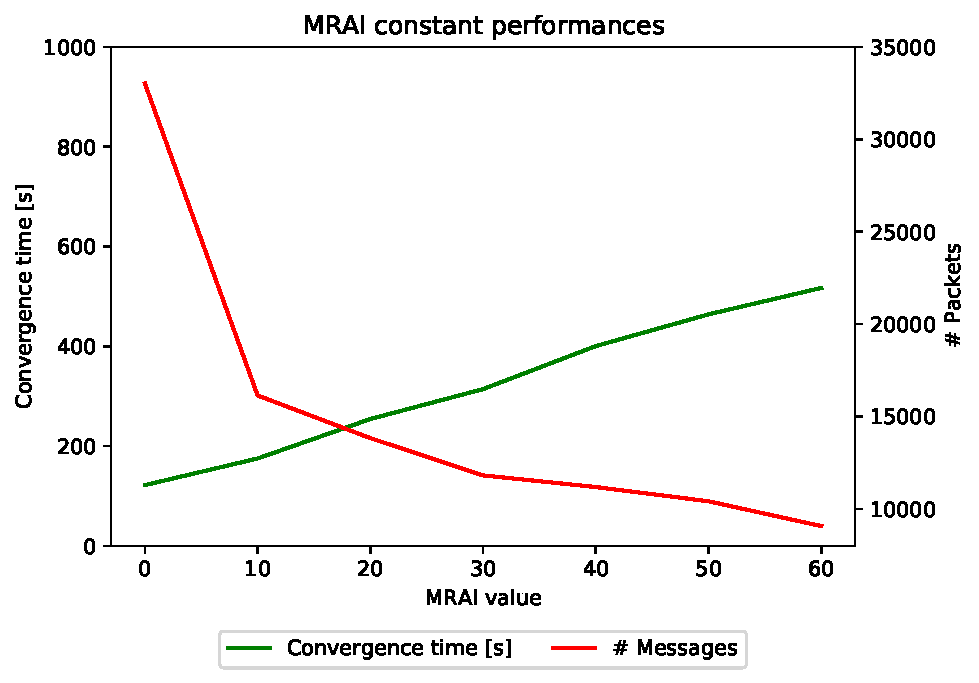
\includegraphics[width=\textwidth]{images/internet_like/1000/signals/AWAW/constant/internet_like-constant_AWAW_mrai_evolution.pdf}
		 \caption{Network perforcances, \textit{fixed} \ac{MRAI} strategy}
         \label{fig:internet_like_1000_fixed_AWAW}
     \end{subfigure}
     \hfill
     \begin{subfigure}[b]{0.45\textwidth}
         \centering
         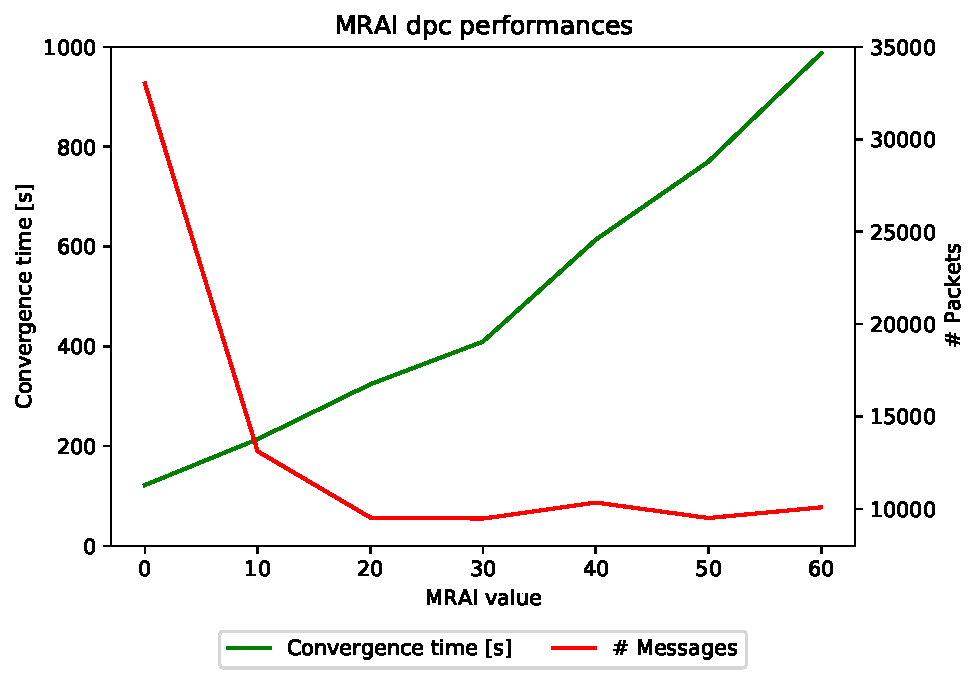
\includegraphics[width=\textwidth]{images/internet_like/1000/signals/AWAW/dpc/internet_like-DPC_AWAW_mrai_evolution.pdf}
		 \caption{Network perforcances, \ac{DPC} \ac{MRAI} strategy}
         \label{fig:internet_like_1000_dpc_AWAW}
     \end{subfigure}
	 \caption{Network perfomances comparison with different \ac{MRAI} strategies,
		Graph internet like with \num{1000} nodes, signal \q{AWAW}}
        \label{fig:internt_like_1000_evolution_AWAW}
\end{figure}

\begin{figure}[h]
     \centering
     \begin{subfigure}[b]{0.45\textwidth}
         \centering
         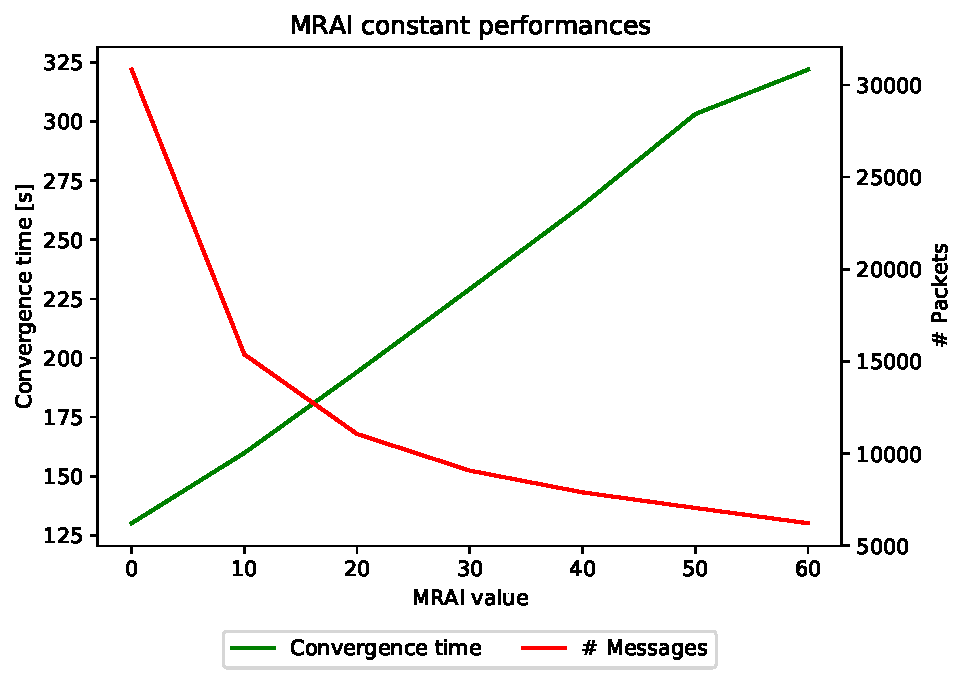
\includegraphics[width=\textwidth]{images/internet_like/1000/signals/AWAWA/constant/internet_like-constant_AWAWA_mrai_evolution.pdf}
		 \caption{Network perforcances, \textit{fixed} \ac{MRAI} strategy}
         \label{fig:internet_like_1000_fixed_AWAWA}
     \end{subfigure}
     \hfill
     \begin{subfigure}[b]{0.45\textwidth}
         \centering
         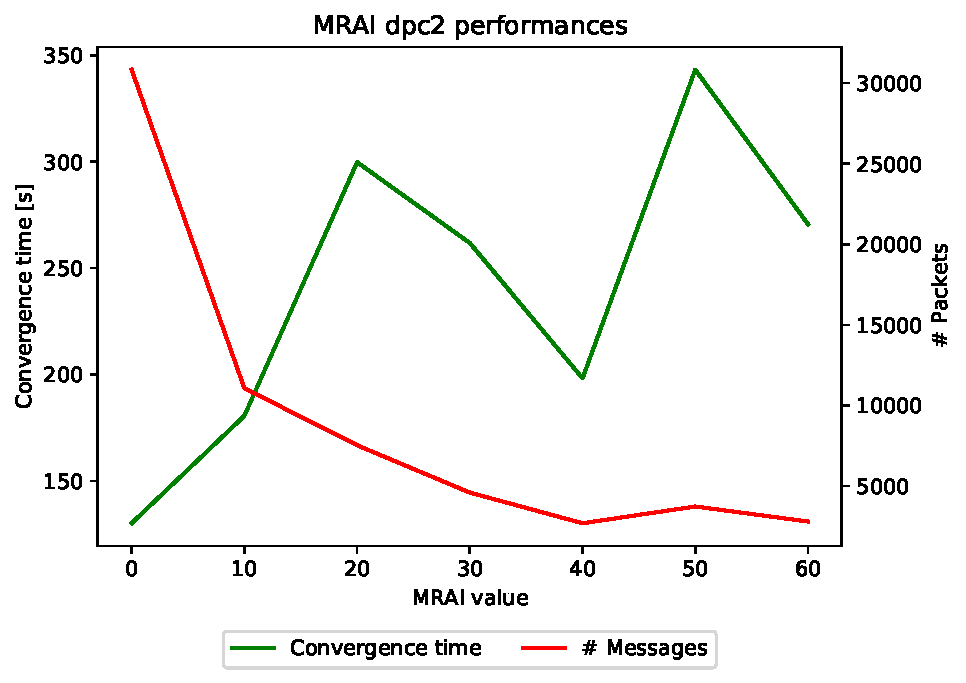
\includegraphics[width=\textwidth]{images/internet_like/1000/signals/AWAWA/dpc/internet_like-DPC_AWAWA_mrai_evolution.pdf}
		 \caption{Network perforcances, \ac{DPC} \ac{MRAI} strategy}
         \label{fig:internet_like_1000_dpc_AWAWA}
     \end{subfigure}
	 \caption{Network perfomances comparison with different \ac{MRAI} strategies,
		Graph internet like with \num{1000} nodes, signal \q{AWAWA}}
        \label{fig:internt_like_1000_evolution_AWAWA}
\end{figure}

\begin{figure}[h]
     \centering
     \begin{subfigure}[b]{0.45\textwidth}
         \centering
         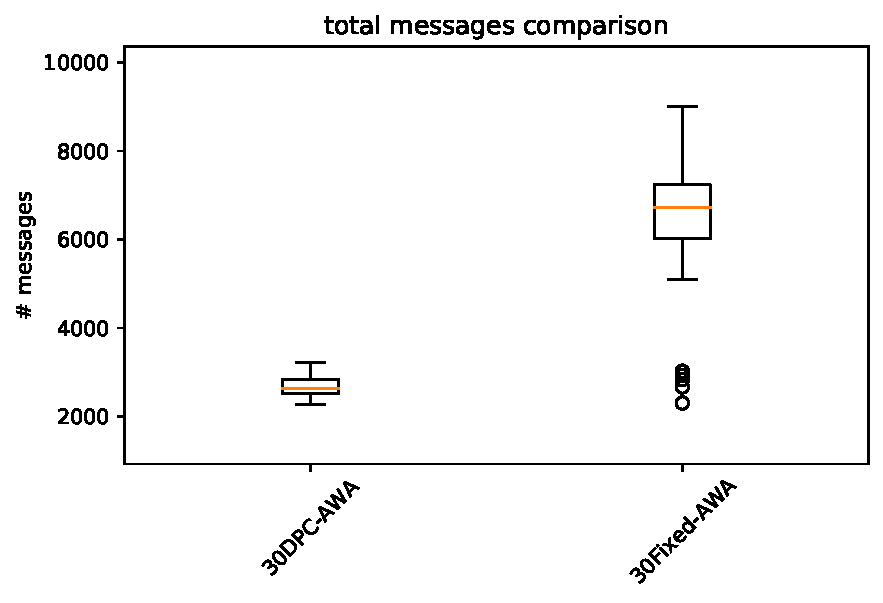
\includegraphics[width=\textwidth]{images/internet_like/1000/comparison/comparison_AWA_messages_boxplot.pdf}
		 \caption{Network perforcances, messages necessary to reach convergence
			with different \ac{MRAI} strategies}
         \label{fig:boxplot_internet_like_1000_messages_AWA}
     \end{subfigure}
     \hfill
     \begin{subfigure}[b]{0.45\textwidth}
         \centering
         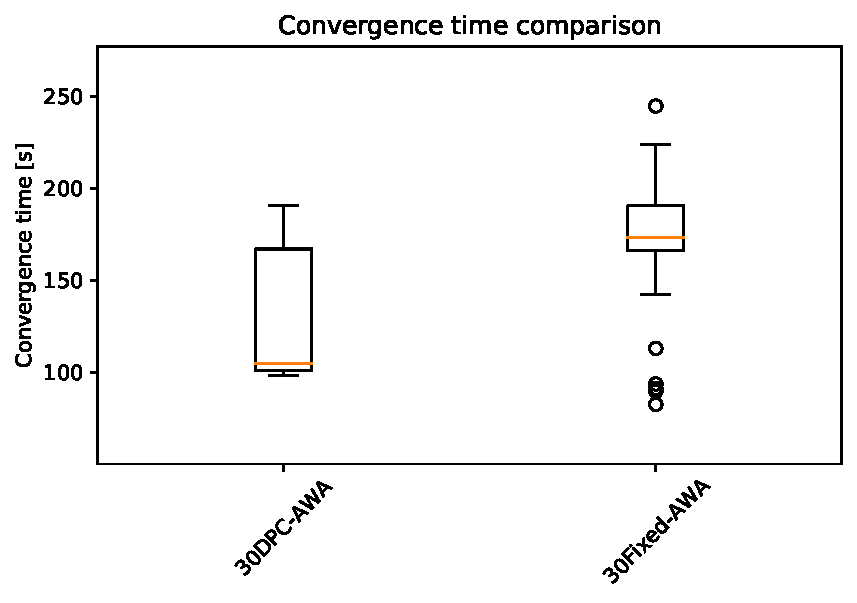
\includegraphics[width=\textwidth]{images/internet_like/1000/comparison/comparison_AWA_time_boxplot.pdf}
		 \caption{Network perforcances, time required to reach convergence
			with different \ac{MRAI} strategies}
         \label{fig:boxplot_internet_like_1000_time_AWA}
     \end{subfigure}
	 \caption{Network perfomances comparison with different \ac{MRAI} strategies,
		Graph internet like with \num{1000} nodes, \ac{MRAI} value 
		\SI{30}{\second}, number of runs for each strategy \num{100}, signal \q{AWA}}
        \label{fig:boxplot_internet_like_1000_AWA}
\end{figure}

\begin{figure}[h]
     \centering
     \begin{subfigure}[b]{0.45\textwidth}
         \centering
         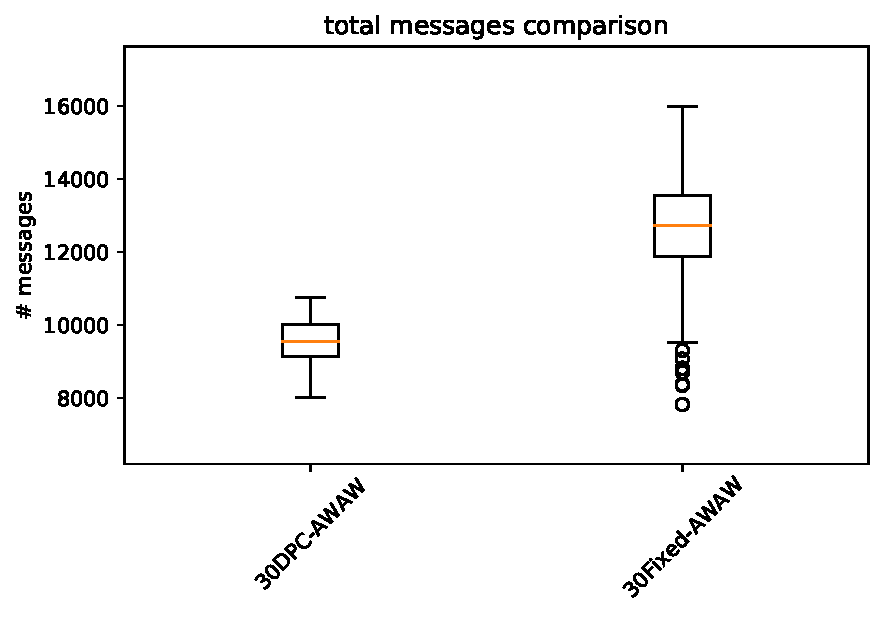
\includegraphics[width=\textwidth]{images/internet_like/1000/comparison/comparison_AWAW_messages_boxplot.pdf}
		 \caption{Network perforcances, messages necessary to reach convergence
			with different \ac{MRAI} strategies}
         \label{fig:boxplot_internet_like_1000_messages_AWAW}
     \end{subfigure}
     \hfill
     \begin{subfigure}[b]{0.45\textwidth}
         \centering
         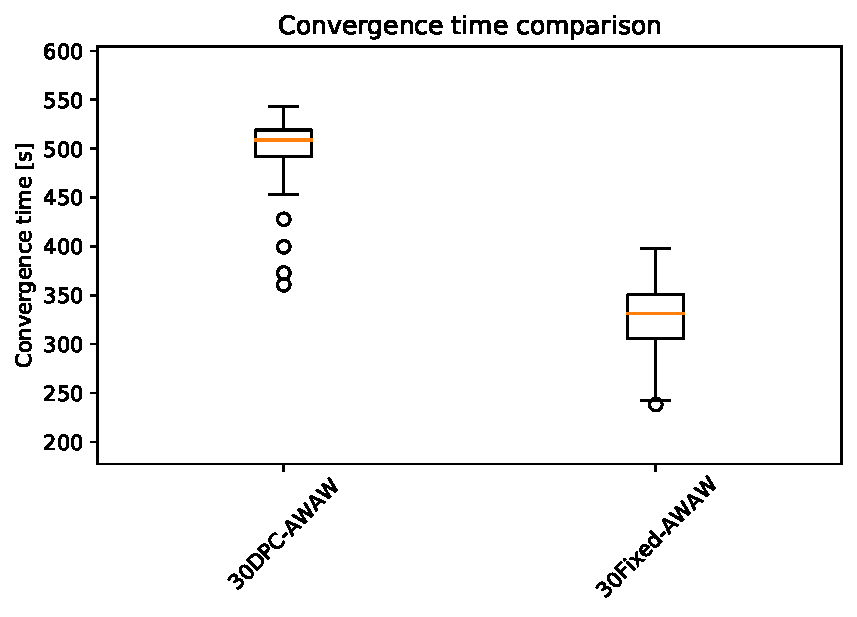
\includegraphics[width=\textwidth]{images/internet_like/1000/comparison/comparison_AWAW_time_boxplot.pdf}
		 \caption{Network perforcances, time required to reach convergence
			with different \ac{MRAI} strategies}
         \label{fig:boxplot_internet_like_1000_time_AWAW}
     \end{subfigure}
	 \caption{Network perfomances comparison with different \ac{MRAI} strategies,
		Graph internet like with \num{1000} nodes, \ac{MRAI} value 
		\SI{30}{\second}, number of runs for each strategy \num{100}, signal \q{AWAW}}
        \label{fig:boxplot_internet_like_1000_AWAW}
\end{figure}

\begin{figure}[h]
     \centering
     \begin{subfigure}[b]{0.45\textwidth}
         \centering
         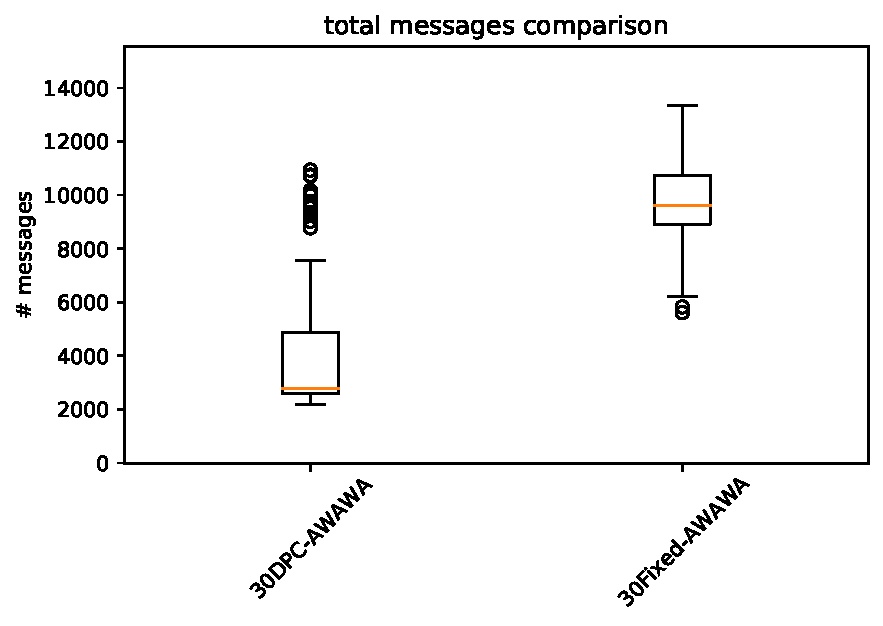
\includegraphics[width=\textwidth]{images/internet_like/1000/comparison/comparison_AWAWA_messages_boxplot.pdf}
		 \caption{Network perforcances, messages necessary to reach convergence
			with different \ac{MRAI} strategies}
         \label{fig:boxplot_internet_like_1000_messages_AWAWA}
     \end{subfigure}
     \hfill
     \begin{subfigure}[b]{0.45\textwidth}
         \centering
         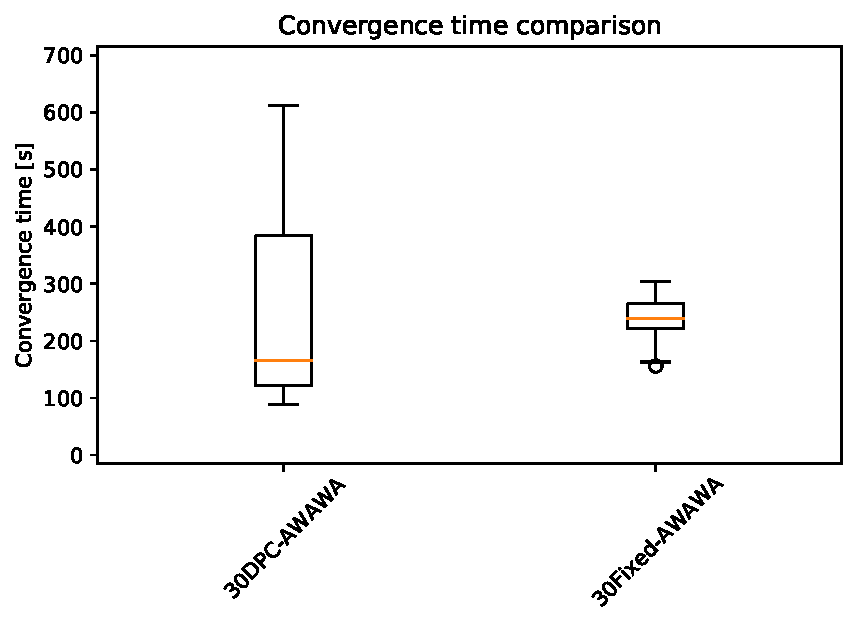
\includegraphics[width=\textwidth]{images/internet_like/1000/comparison/comparison_AWAWA_time_boxplot.pdf}
		 \caption{Network perforcances, time required to reach convergence
			with different \ac{MRAI} strategies}
         \label{fig:boxplot_internet_like_1000_time_AWAWA}
     \end{subfigure}
	 \caption{Network perfomances comparison with different \ac{MRAI} strategies,
		Graph internet like with \num{1000} nodes, \ac{MRAI} value 
		\SI{30}{\second}, number of runs for each strategy \num{100}, signal \q{AWAWA}}
        \label{fig:boxplot_internet_like_1000_AWAWA}
\end{figure}

\begin{figure}[h]
    \centering
    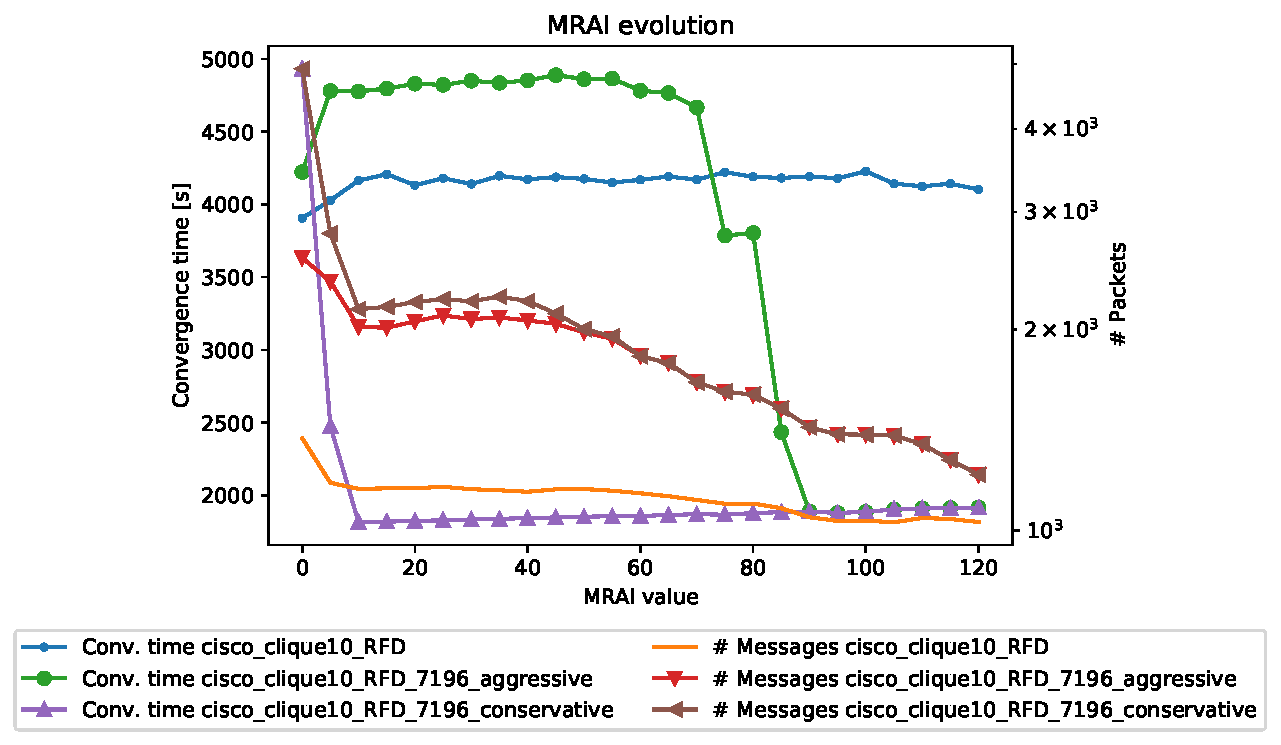
\includegraphics[width=\textwidth]{images/RFD/clique/cisco_clique10_RFD_comparison_constant_all.pdf}
	\caption{Comparison of the \textit{clique} topology with RFD 2439 and the with 
		RFD 7196 strategies}
    \label{fig:clique_RFD2439VSRFD7196}
\end{figure}

\begin{figure}[h]
     \centering
     \begin{subfigure}[b]{0.3\textwidth}
         \centering
         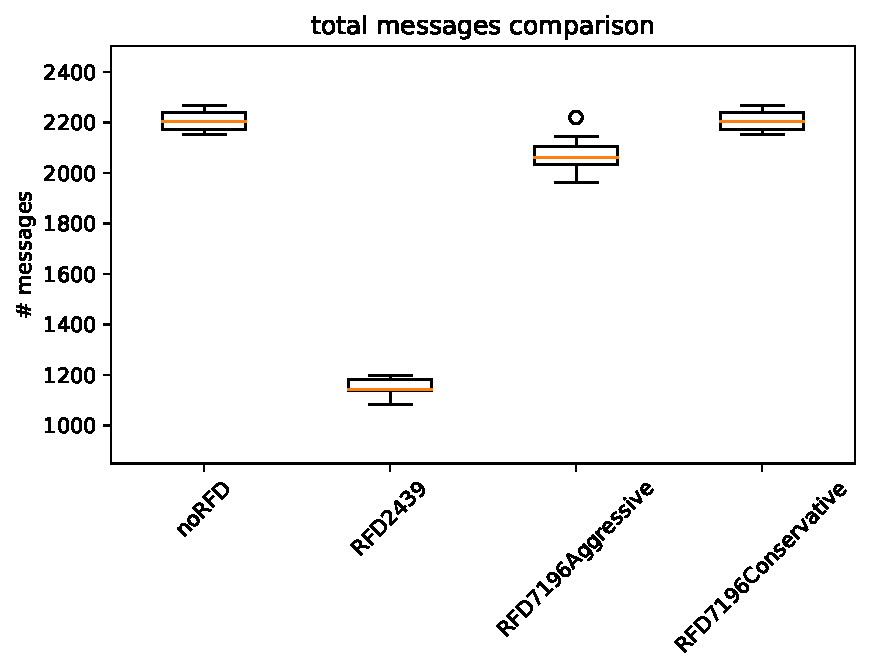
\includegraphics[width=\textwidth]{images/RFD/clique/clique_rfd_comparison_messages_boxplot.pdf}
         \caption{clique topology, MRAI=30s, 10 runs, Messages comparison}
         \label{fig:RFD_MRAI30_messages}
     \end{subfigure}
     \hfill
     \begin{subfigure}[b]{0.3\textwidth}
         \centering
         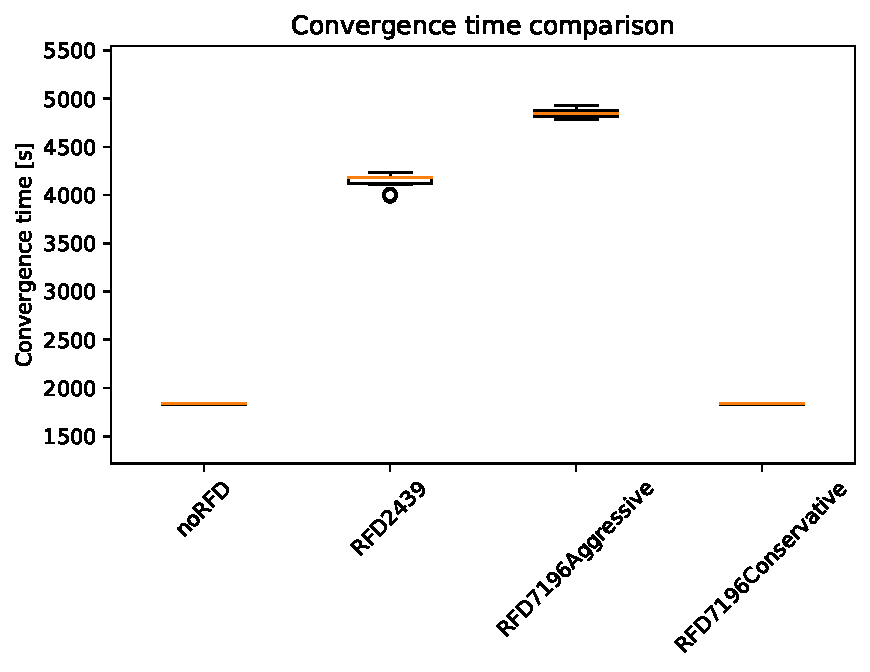
\includegraphics[width=\textwidth]{images/RFD/clique/clique_rfd_comparison_time_boxplot.pdf}
         \caption{clique topology, MRAI=30s, 10 runs, Convergence time}
         \label{fig:RFD_MRAI30_convTime}
     \end{subfigure}
     \hfill
     \begin{subfigure}[b]{0.3\textwidth}
         \centering
         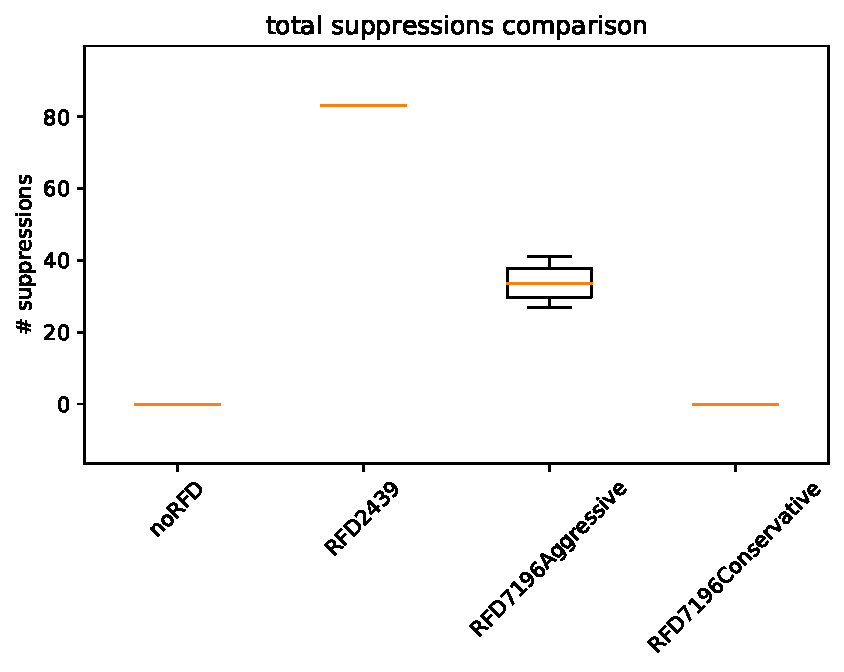
\includegraphics[width=\textwidth]{images/RFD/clique/clique_rfd_comparison_suppressions_boxplot.pdf}
         \caption{clique topology, MRAI=30s, 10 runs, Number of suppressions}
         \label{fig:RFD_MRAI30_suppressions}
     \end{subfigure}
        \caption{Clique topology, MRAI=30s, 10 runs, comparison of the network performances}
        \label{fig:RFD_MRAI30}
\end{figure}
\clearpage

\begin{figure}[H]
     \centering
     \begin{subfigure}[b]{0.325\textwidth}
         \centering
         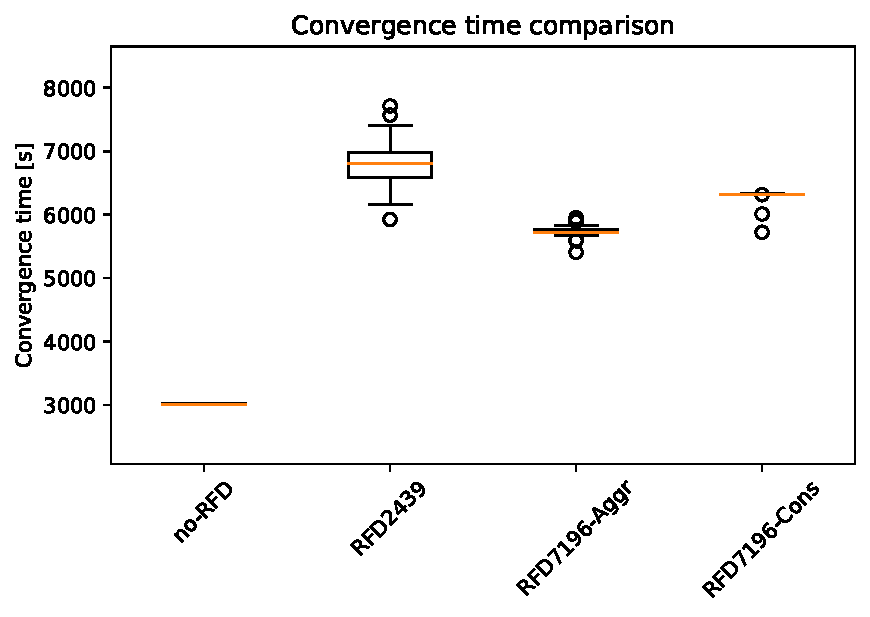
\includegraphics[width=\textwidth]{images/RFD/miceVSelephants/MultiMRAI/0/mice/cisco_1000MRAI0_rfd_comparison_time_boxplot.pdf}
         \caption{Convergence time respect to the RFD strategy, MRAI=0s}
         \label{fig:1000_RFD_MRAI0_time_mice}
     \end{subfigure}
     \hfill
     \begin{subfigure}[b]{0.325\textwidth}
         \centering
         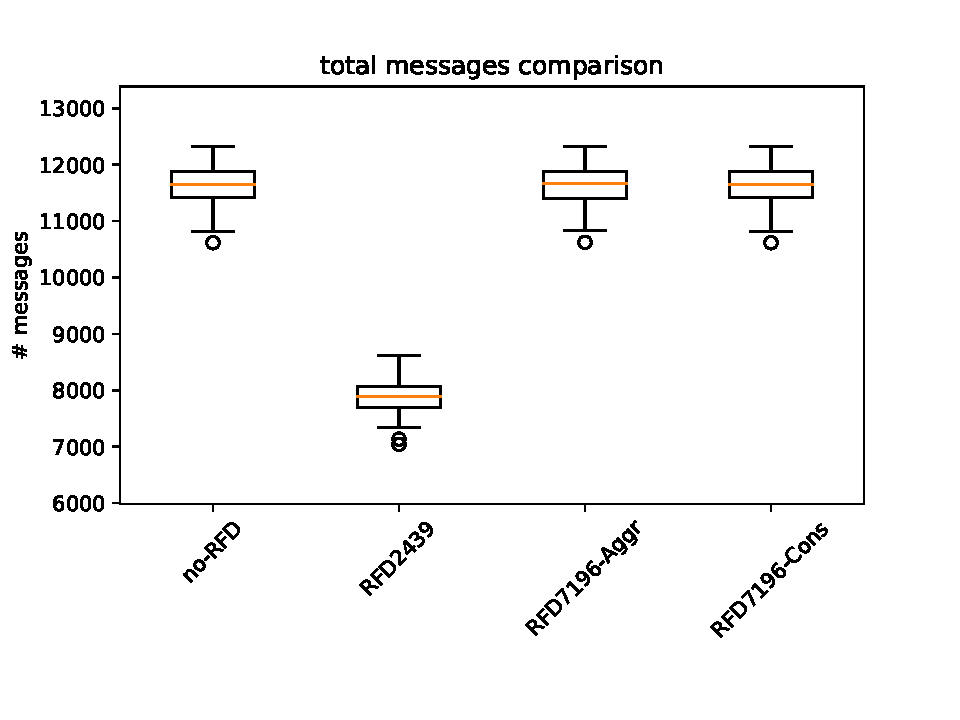
\includegraphics[width=\textwidth]{images/RFD/miceVSelephants/MultiMRAI/0/mice/cisco_1000MRAI0_rfd_comparison_messages_boxplot.pdf}
         \caption{Number of messages respect to the RFD strategy, MRAI=0s}
         \label{fig:1000_RFD_MRAI0_messages_mice}
     \end{subfigure}
     \hfill
     \begin{subfigure}[b]{0.325\textwidth}
         \centering
         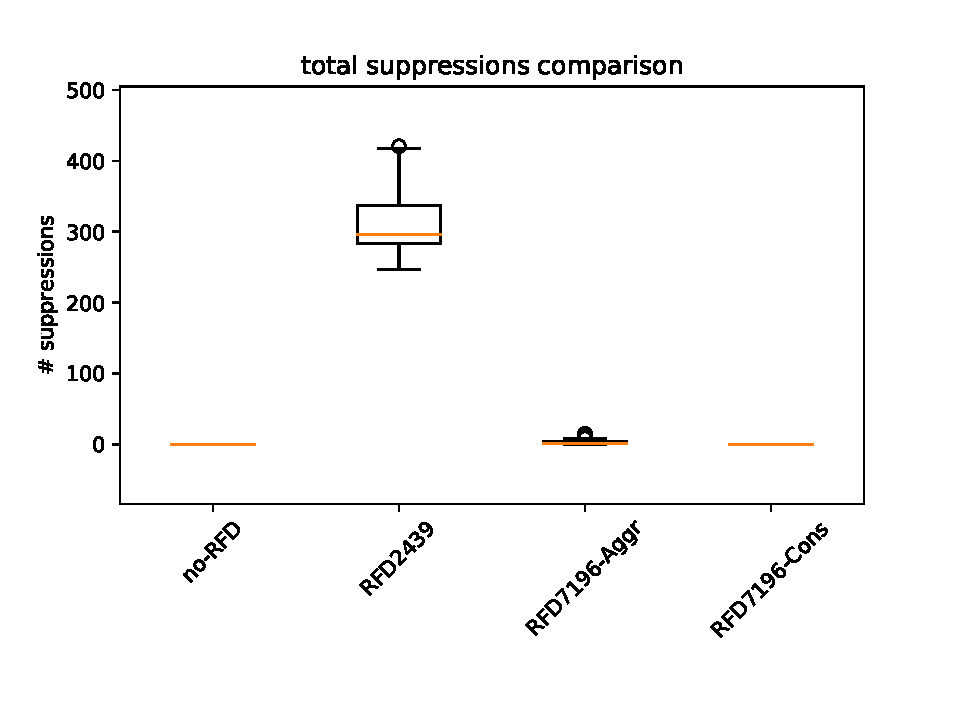
\includegraphics[width=\textwidth]{images/RFD/miceVSelephants/MultiMRAI/0/mice/cisco_1000MRAI0_rfd_comparison_suppressions_boxplot.pdf}
         \caption{Number of suppressions respect to the RFD strategy, MRAI=0s}
         \label{fig:1000_RFD_MRAI0_suppressions_mice}
     \end{subfigure}
     \vfill
     \begin{subfigure}[b]{0.325\textwidth}
         \centering
         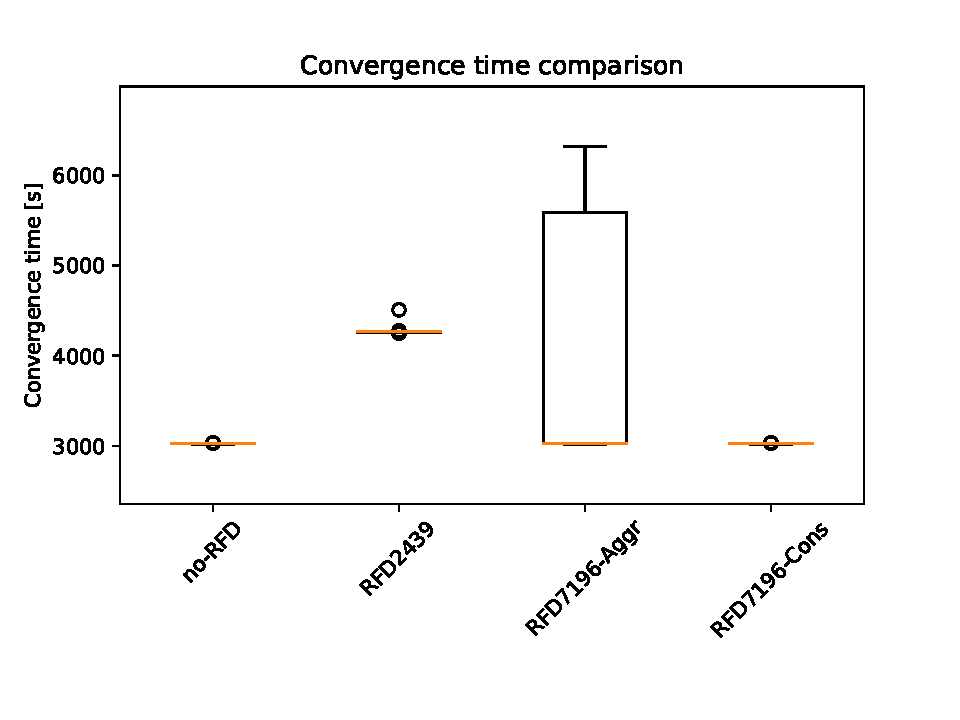
\includegraphics[width=\textwidth]{images/RFD/miceVSelephants/MultiMRAI/15/mice/cisco_1000MRAI15_rfd_comparison_time_boxplot.pdf}
         \caption{Convergence time respect to the RFD strategy, MRAI=15s}
         \label{fig:1000_RFD_MRAI15_time_mice}
     \end{subfigure}
     \hfill
     \begin{subfigure}[b]{0.325\textwidth}
         \centering
         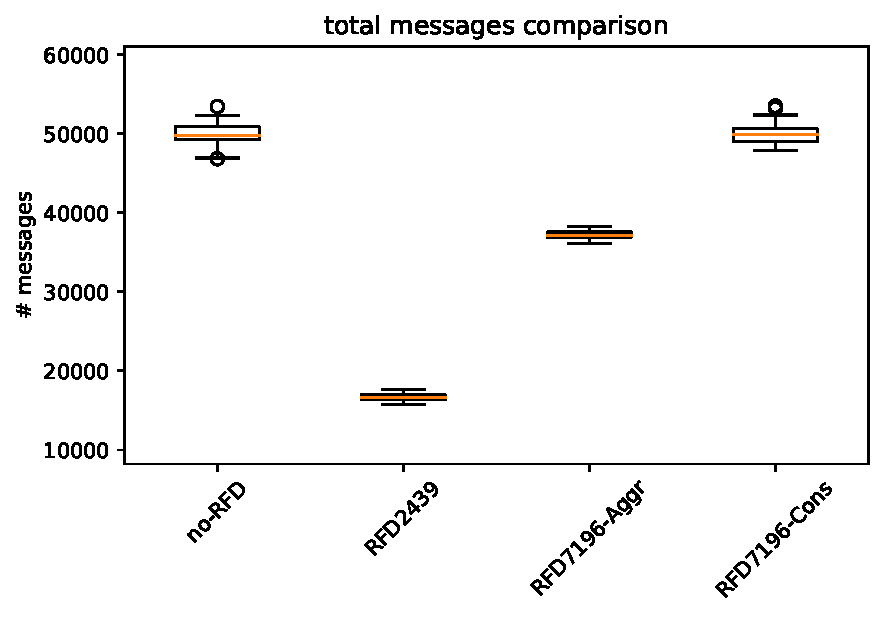
\includegraphics[width=\textwidth]{images/RFD/miceVSelephants/MultiMRAI/15/mice/cisco_1000MRAI15_rfd_comparison_messages_boxplot.pdf}
         \caption{Number of messages respect to the RFD strategy, MRAI=15s}
         \label{fig:1000_RFD_MRAI15_messages_mice}
     \end{subfigure}
     \hfill
     \begin{subfigure}[b]{0.325\textwidth}
         \centering
         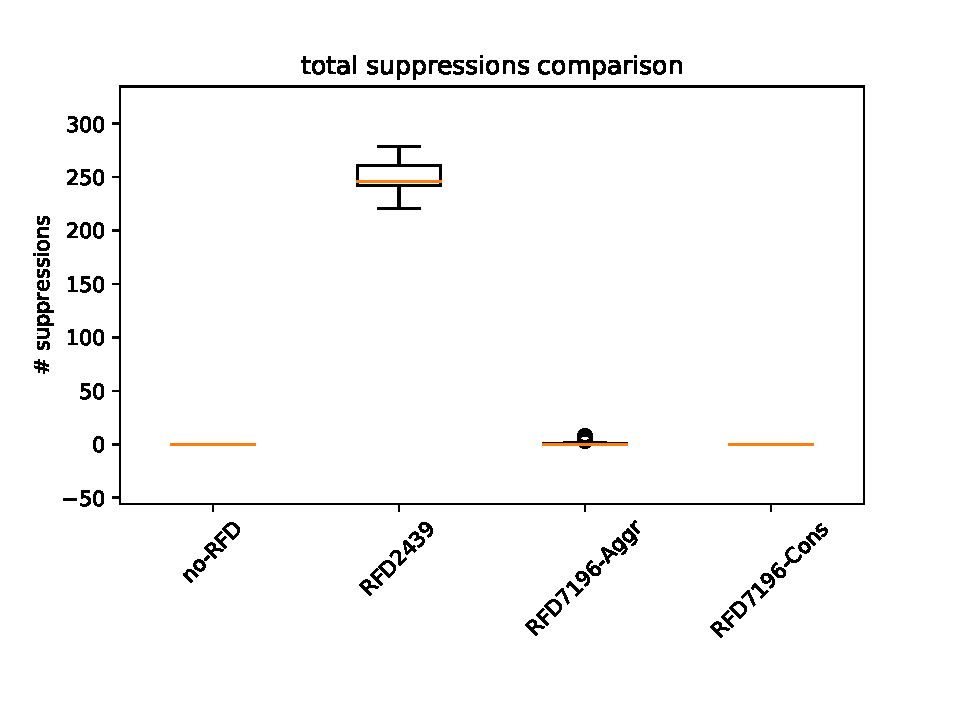
\includegraphics[width=\textwidth]{images/RFD/miceVSelephants/MultiMRAI/15/mice/cisco_1000MRAI15_rfd_comparison_suppressions_boxplot.pdf}
         \caption{Number of suppressions respect to the RFD strategy, MRAI=15s}
         \label{fig:1000_RFD_MRAI15_suppressions_mice}
     \end{subfigure}
     \vfill
     \begin{subfigure}[b]{0.325\textwidth}
         \centering
         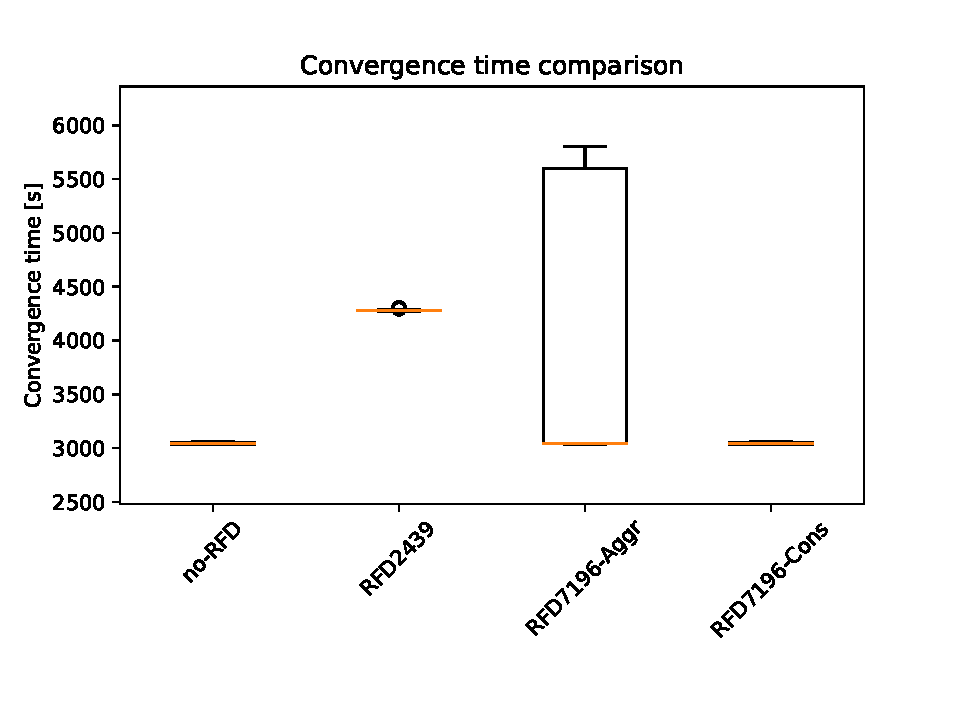
\includegraphics[width=\textwidth]{images/RFD/miceVSelephants/MultiMRAI/30/mice/cisco_1000MRAI30_rfd_comparison_time_boxplot.pdf}
         \caption{Convergence time respect to the RFD strategy, MRAI=30s}
         \label{fig:1000_RFD_MRAI30_time_mice}
     \end{subfigure}
     \hfill
     \begin{subfigure}[b]{0.325\textwidth}
         \centering
         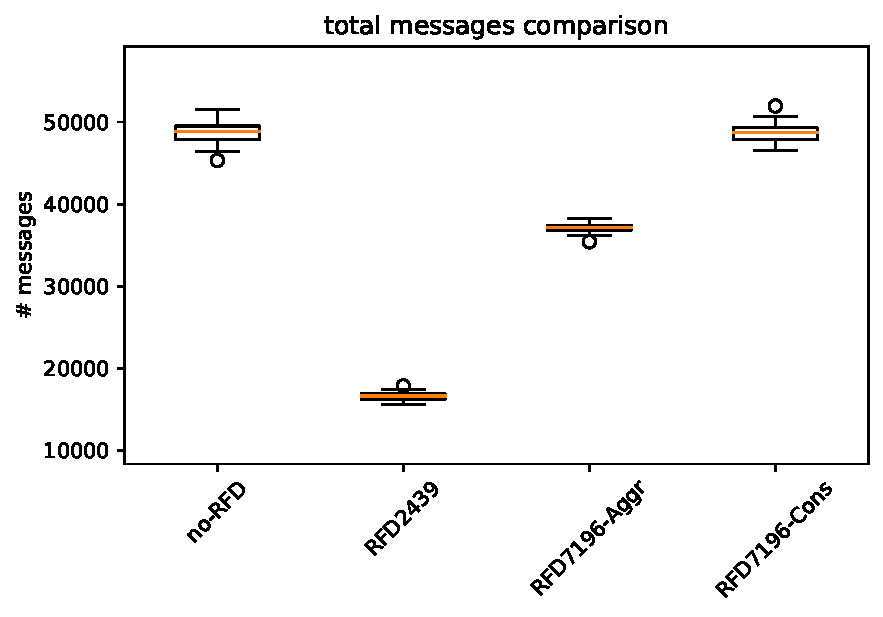
\includegraphics[width=\textwidth]{images/RFD/miceVSelephants/MultiMRAI/30/mice/cisco_1000MRAI30_rfd_comparison_messages_boxplot.pdf}
         \caption{Number of messages respect to the RFD strategy, MRAI=30s}
         \label{fig:1000_RFD_MRAI30_messages_mice}
     \end{subfigure}
     \hfill
     \begin{subfigure}[b]{0.325\textwidth}
         \centering
         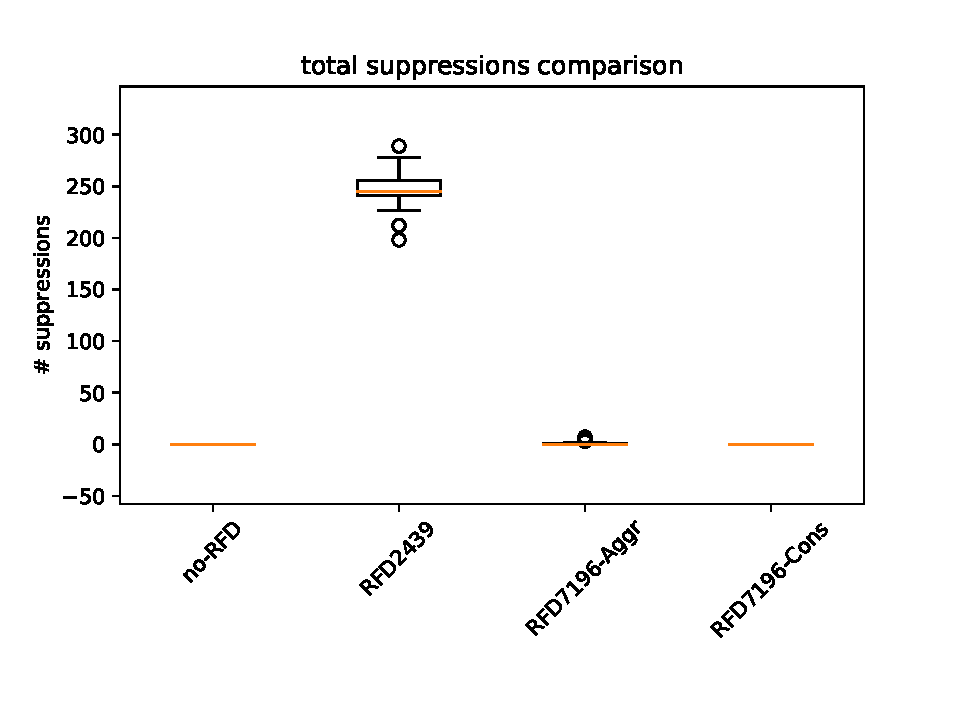
\includegraphics[width=\textwidth]{images/RFD/miceVSelephants/MultiMRAI/30/mice/cisco_1000MRAI30_rfd_comparison_suppressions_boxplot.pdf}
         \caption{Number of suppressions respect to the RFD strategy, MRAI=30s}
         \label{fig:1000_RFD_MRAI30_suppressions_mice}
     \end{subfigure}
     \vfill
     \begin{subfigure}[b]{0.325\textwidth}
         \centering
         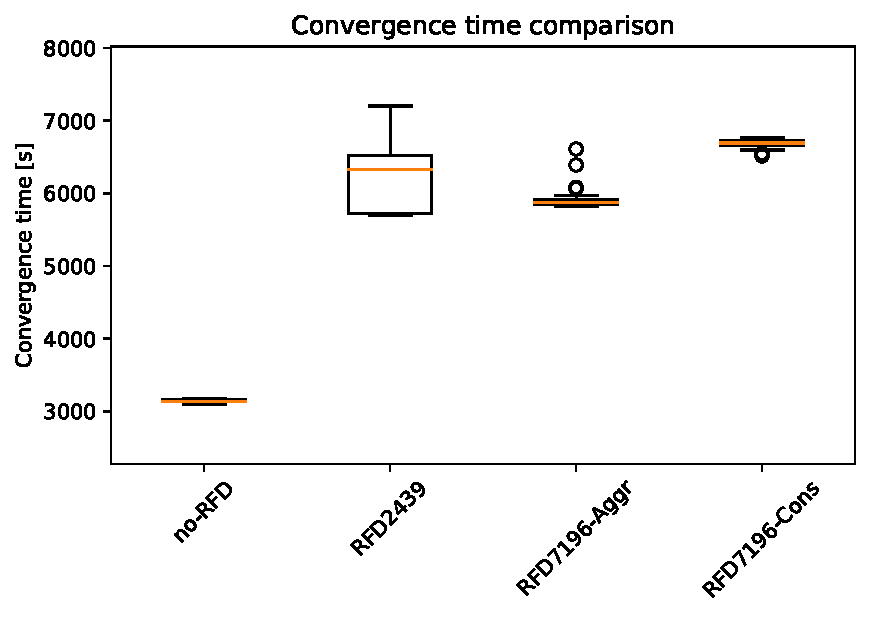
\includegraphics[width=\textwidth]{images/RFD/miceVSelephants/MultiMRAI/45/mice/cisco_1000MRAI45_rfd_comparison_time_boxplot.pdf}
         \caption{Convergence time respect to the RFD strategy, MRAI=45s}
         \label{fig:1000_RFD_MRAI45_time_mice}
     \end{subfigure}
     \hfill
     \begin{subfigure}[b]{0.325\textwidth}
         \centering
         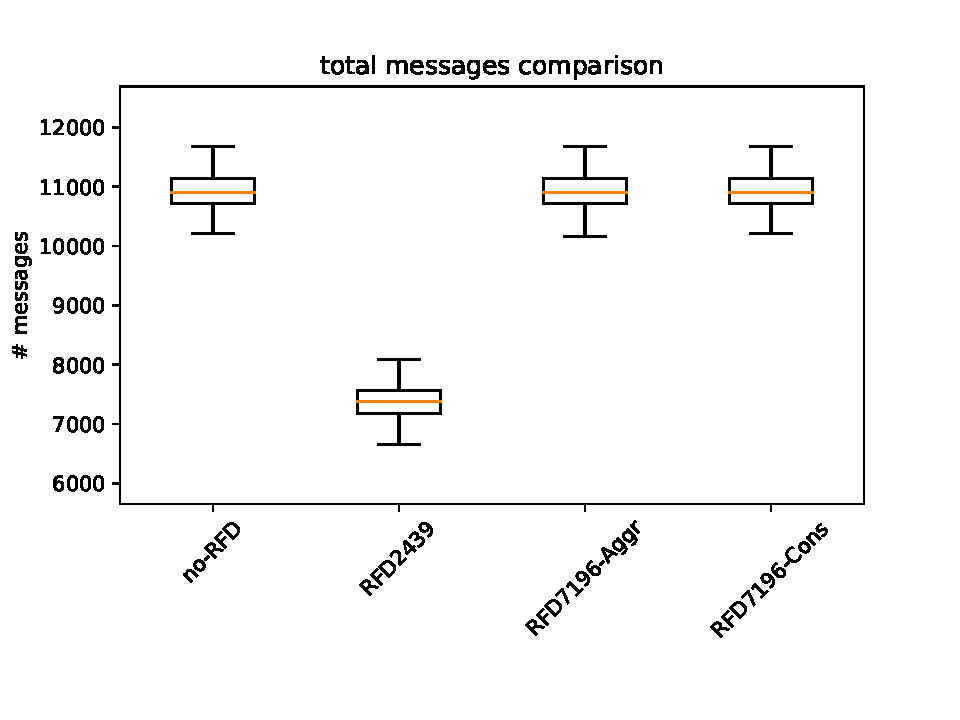
\includegraphics[width=\textwidth]{images/RFD/miceVSelephants/MultiMRAI/45/mice/cisco_1000MRAI45_rfd_comparison_messages_boxplot.pdf}
         \caption{Number of messages respect to the RFD strategy, MRAI=30s}
         \label{fig:1000_RFD_MRAI45_messages_mice}
     \end{subfigure}
     \hfill
     \begin{subfigure}[b]{0.325\textwidth}
         \centering
         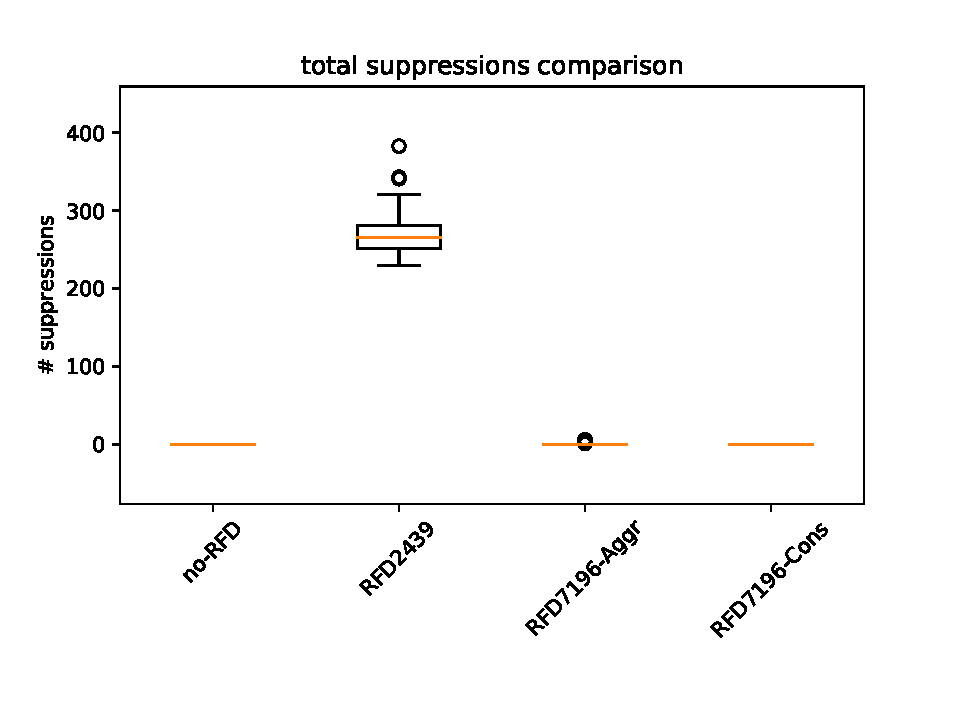
\includegraphics[width=\textwidth]{images/RFD/miceVSelephants/MultiMRAI/45/mice/cisco_1000MRAI45_rfd_comparison_suppressions_boxplot.pdf}
         \caption{Number of suppressions respect to the RFD strategy, MRAI=45s}
         \label{fig:1000_RFD_MRAI45_suppressions_mice}
     \end{subfigure}
     \vfill
     \begin{subfigure}[b]{0.325\textwidth}
         \centering
         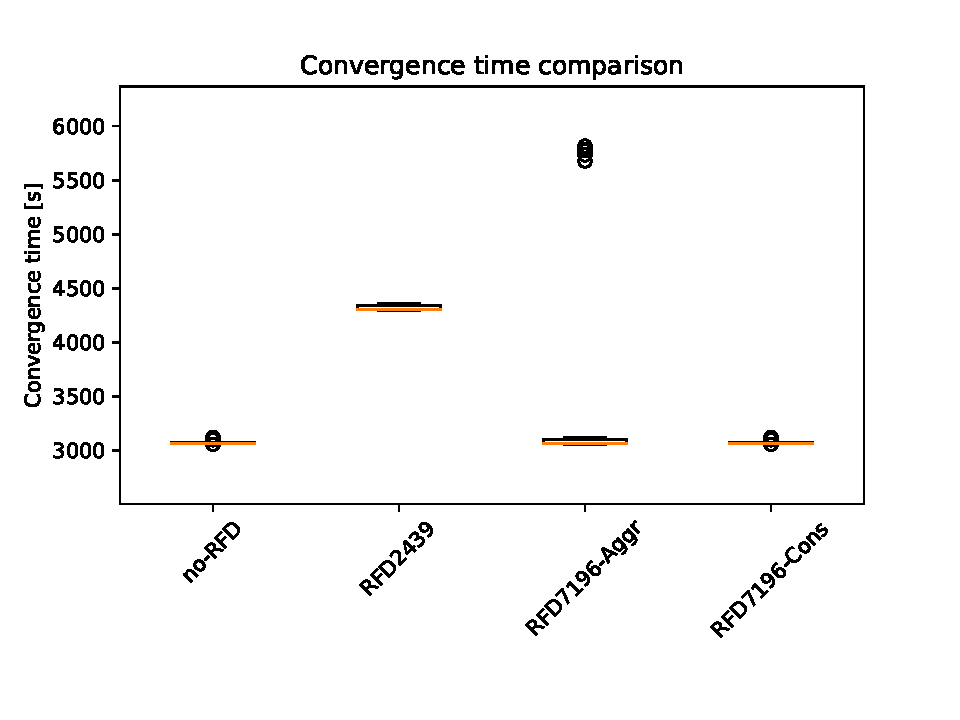
\includegraphics[width=\textwidth]{images/RFD/miceVSelephants/MultiMRAI/60/mice/cisco_1000MRAI60_rfd_comparison_time_boxplot.pdf}
         \caption{Convergence time respect to the RFD strategy, MRAI=60s}
         \label{fig:1000_RFD_MRAI60_time_mice}
     \end{subfigure}
     \hfill
     \begin{subfigure}[b]{0.325\textwidth}
         \centering
         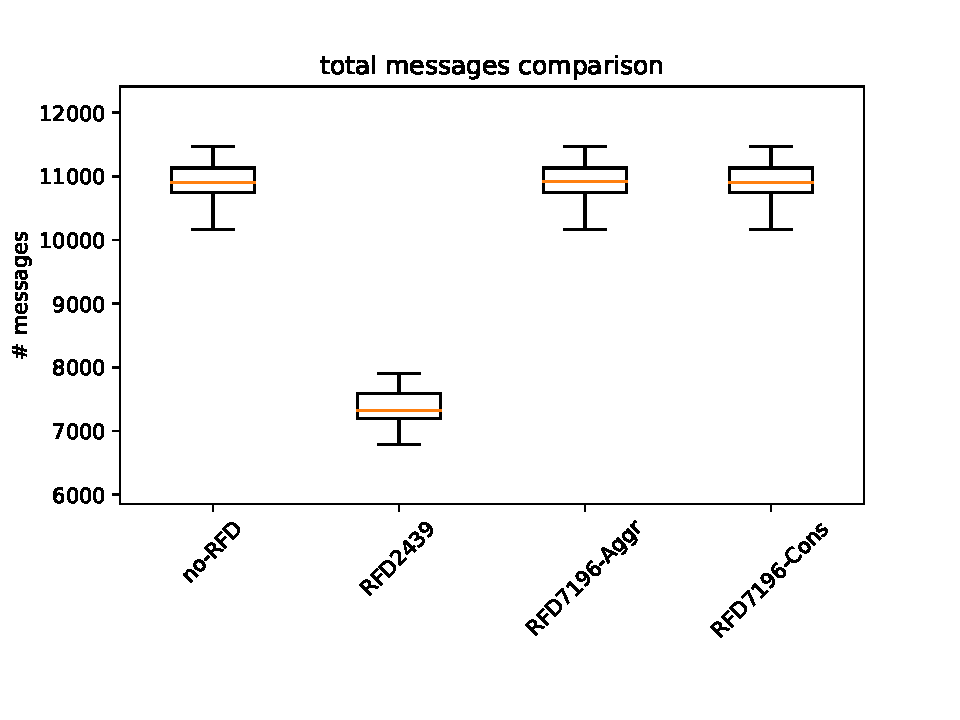
\includegraphics[width=\textwidth]{images/RFD/miceVSelephants/MultiMRAI/60/mice/cisco_1000MRAI60_rfd_comparison_messages_boxplot.pdf}
         \caption{Number of messages respect to the RFD strategy, MRAI=60s}
         \label{fig:1000_RFD_MRAI60_messages_mice}
     \end{subfigure}
     \hfill
     \begin{subfigure}[b]{0.325\textwidth}
         \centering
         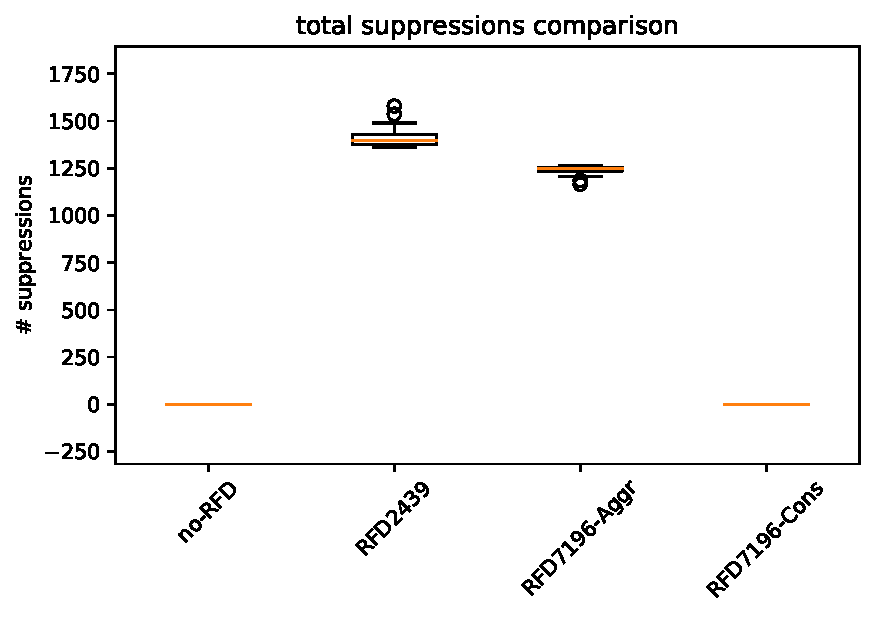
\includegraphics[width=\textwidth]{images/RFD/miceVSelephants/MultiMRAI/60/mice/cisco_1000MRAI60_rfd_comparison_suppressions_boxplot.pdf}
         \caption{Number of suppressions respect to the RFD strategy, MRAI=60s}
         \label{fig:1000_RFD_MRAI60_suppressions_mice}
     \end{subfigure}
        \caption{Internet like topology 1000 nodes, random destination, 5 flaps, 300s delay, Network performances}
        \label{fig:1000_RFD_MRAI30_mice}
\end{figure}

\begin{figure}[H]
     \centering
     \begin{subfigure}[b]{0.325\textwidth}
         \centering
         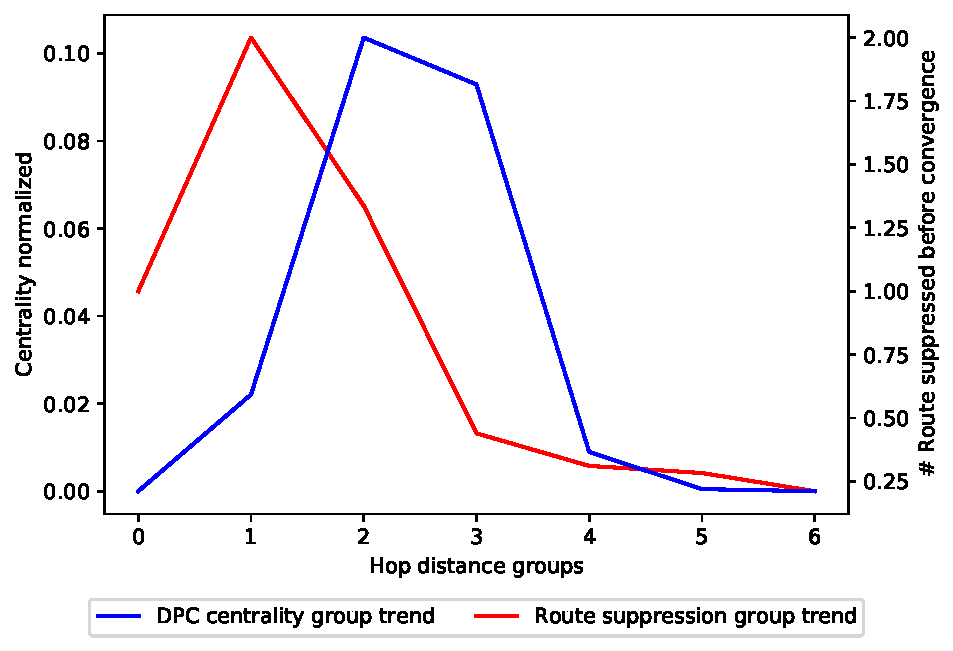
\includegraphics[width=\textwidth]{images/RFD/miceVSelephants/MultiMRAI/0/mice/cisco_1000_RFD_nodeConvergence_centVSsup_trend.pdf}
         \caption{RFD 2439 Strategy, \\MRAI=0s}
         \label{fig:1000_2439RFD_centVSsup_mices_MRAI0}
     \end{subfigure}
     \hfill
     \begin{subfigure}[b]{0.325\textwidth}
         \centering
         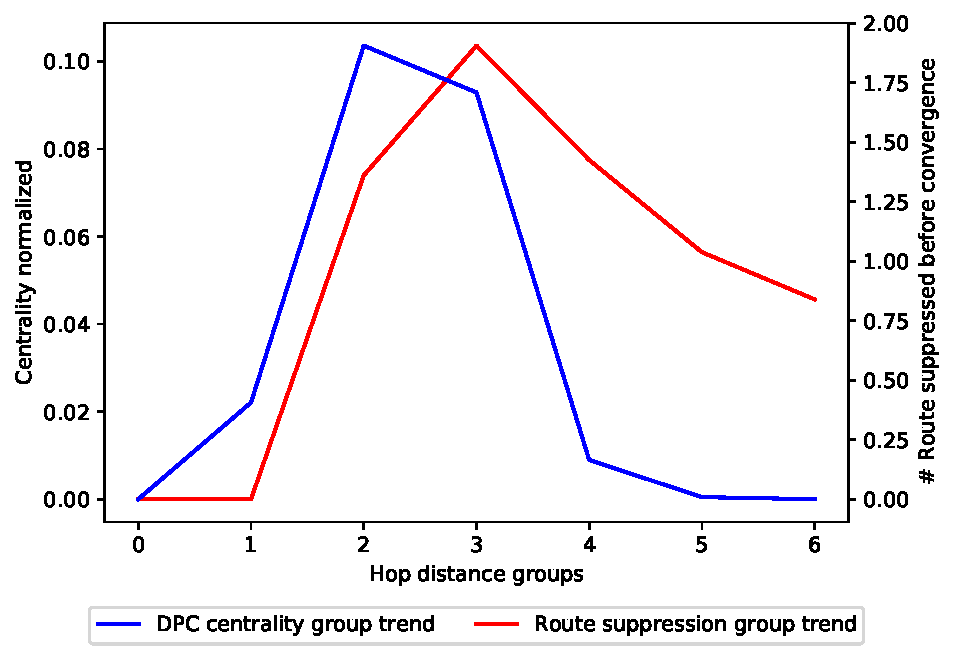
\includegraphics[width=\textwidth]{images/RFD/miceVSelephants/MultiMRAI/0/mice/cisco_1000_RFD_7196_aggressive_nodeConvergence_centVSsup_trend.pdf}
         \caption{RFD 7196 Aggressive Strategy, MRAI=0s}
         \label{fig:1000_7196RFDA_centVSsup_mices_MRAI0}
     \end{subfigure}
     \hfill
     \begin{subfigure}[b]{0.325\textwidth}
         \centering
         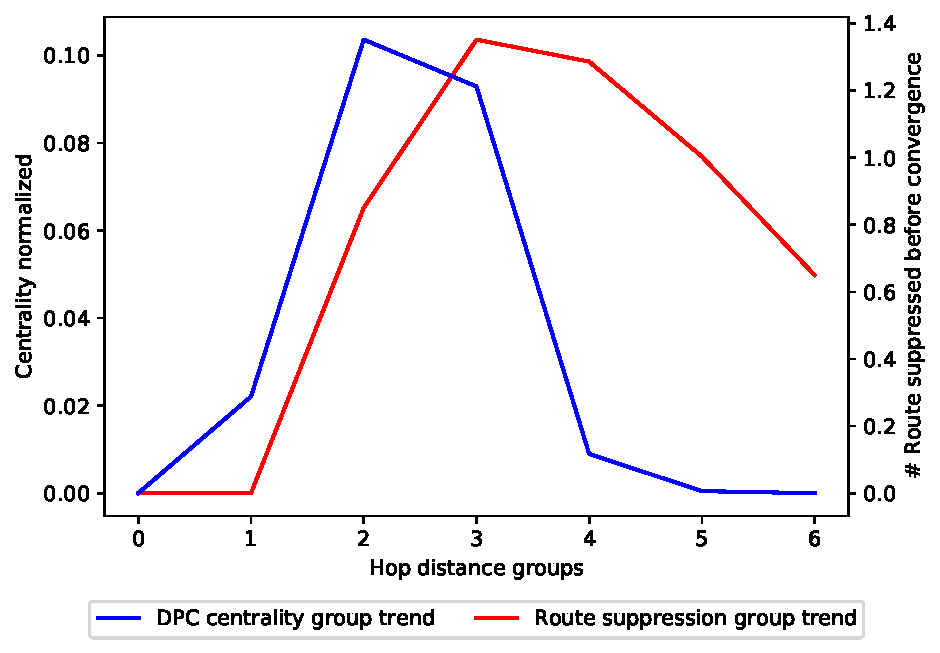
\includegraphics[width=\textwidth]{images/RFD/miceVSelephants/MultiMRAI/0/mice/cisco_1000_RFD_7196_conservative_nodeConvergence_centVSsup_trend.pdf}
         \caption{RFD 7196 Conservative Strategy, MRAI=0s}
         \label{fig:1000_7196RFDC_centVSsup_mices_MRAI0}
     \end{subfigure}
     \vfill
     \begin{subfigure}[b]{0.325\textwidth}
         \centering
         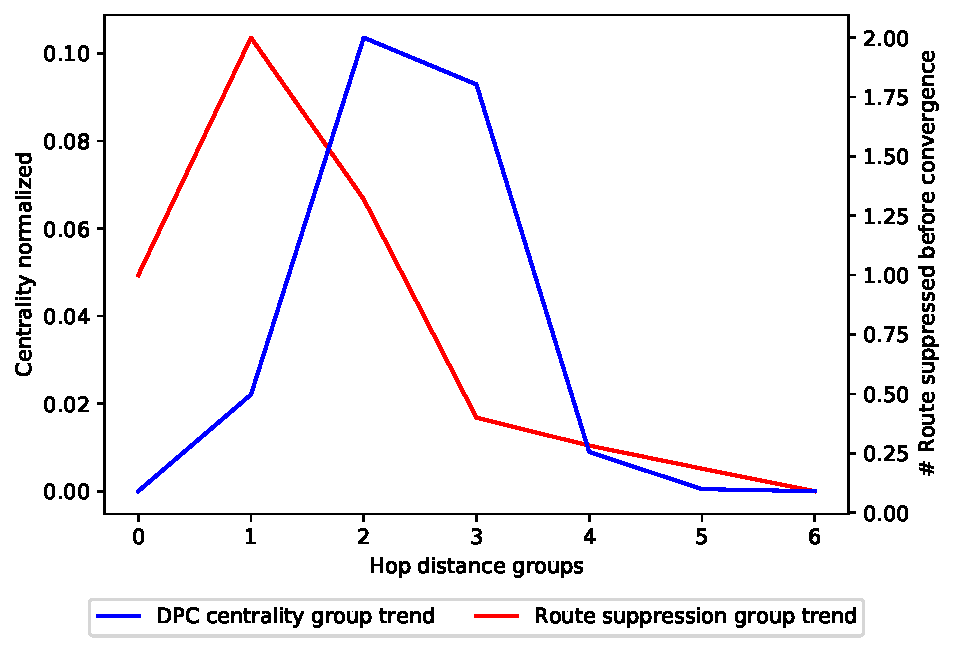
\includegraphics[width=\textwidth]{images/RFD/miceVSelephants/MultiMRAI/15/mice/cisco_1000_RFD_nodeConvergence_centVSsup_trend.pdf}
         \caption{RFD 2439 Strategy, \\MRAI=15s}
         \label{fig:1000_2439RFD_centVSsup_mices_MRAI15}
     \end{subfigure}
     \hfill
     \begin{subfigure}[b]{0.325\textwidth}
         \centering
         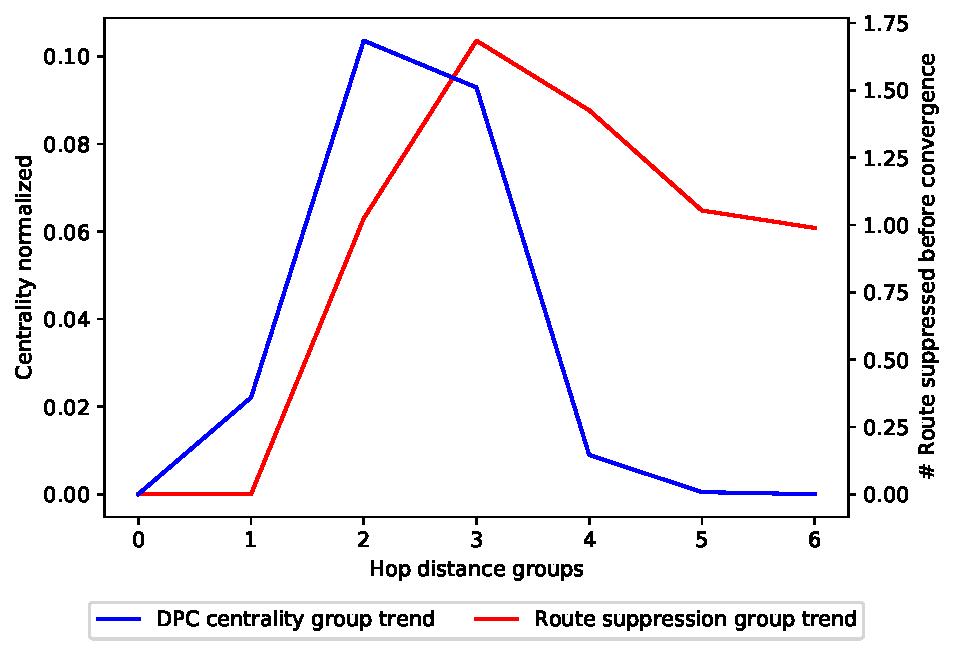
\includegraphics[width=\textwidth]{images/RFD/miceVSelephants/MultiMRAI/15/mice/cisco_1000_RFD_7196_aggressive_nodeConvergence_centVSsup_trend.pdf}
         \caption{RFD 7196 Aggressive Strategy, MRAI=15s}
         \label{fig:1000_7196RFDA_centVSsup_mices_MRAI15}
     \end{subfigure}
     \hfill
     \begin{subfigure}[b]{0.325\textwidth}
         \centering
         \includegraphics[width=\textwidth]{images/RFD/miceVSelephants/MultiMRAI/15/mice/cisco_1000_RFD_7196_conservative_nodeConvergence_centVSsup_trend.pdf}
         \caption{RFD 7196 Conservative Strategy, MRAI=15s}
         \label{fig:1000_7196RFDC_centVSsup_mices_MRAI15}
     \end{subfigure}
     \vfill
     \begin{subfigure}[b]{0.325\textwidth}
         \centering
         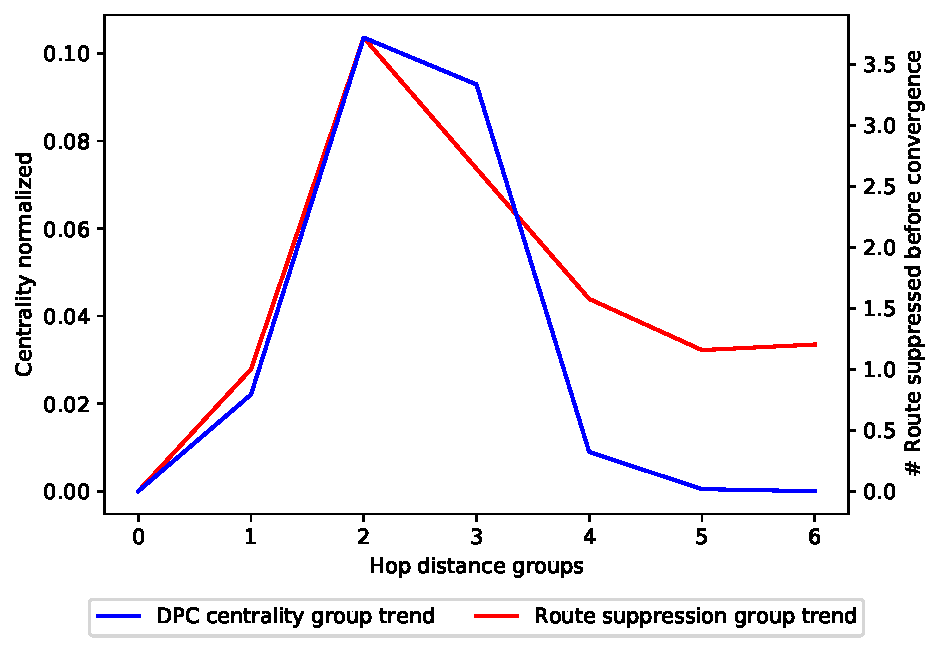
\includegraphics[width=\textwidth]{images/RFD/miceVSelephants/MultiMRAI/30/mice/cisco_1000_RFD_nodeConvergence_centVSsup_trend.pdf}
         \caption{RFD 2439 Strategy, \\MRAI=30s}
         \label{fig:1000_2439RFD_centVSsup_mices_MRAI30}
     \end{subfigure}
     \hfill
     \begin{subfigure}[b]{0.325\textwidth}
         \centering
         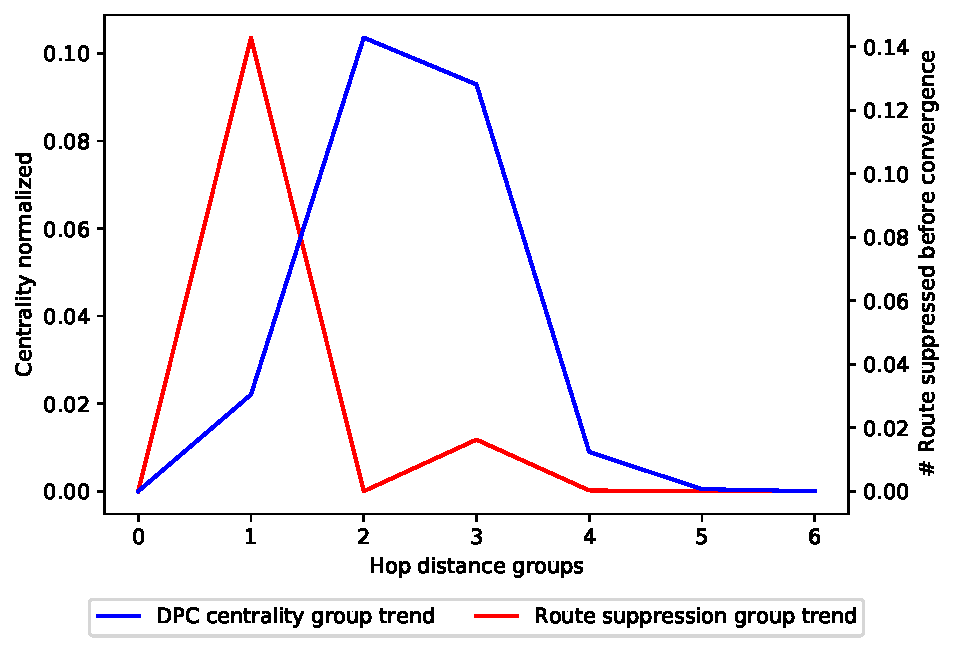
\includegraphics[width=\textwidth]{images/RFD/miceVSelephants/MultiMRAI/30/mice/cisco_1000_RFD_7196_aggressive_nodeConvergence_centVSsup_trend.pdf}
         \caption{RFD 7196 Aggressive Strategy, MRAI=30s}
         \label{fig:1000_7196RFDA_centVSsup_mices_MRAI30}
     \end{subfigure}
     \hfill
     \begin{subfigure}[b]{0.325\textwidth}
         \centering
         \includegraphics[width=\textwidth]{images/RFD/miceVSelephants/MultiMRAI/30/mice/cisco_1000_RFD_7196_conservative_nodeConvergence_centVSsup_trend.pdf}
         \caption{RFD 7196 Conservative Strategy, MRAI=30s}
         \label{fig:1000_7196RFDC_centVSsup_mices_MRAI30}
     \end{subfigure}
     \vfill
     \begin{subfigure}[b]{0.325\textwidth}
         \centering
         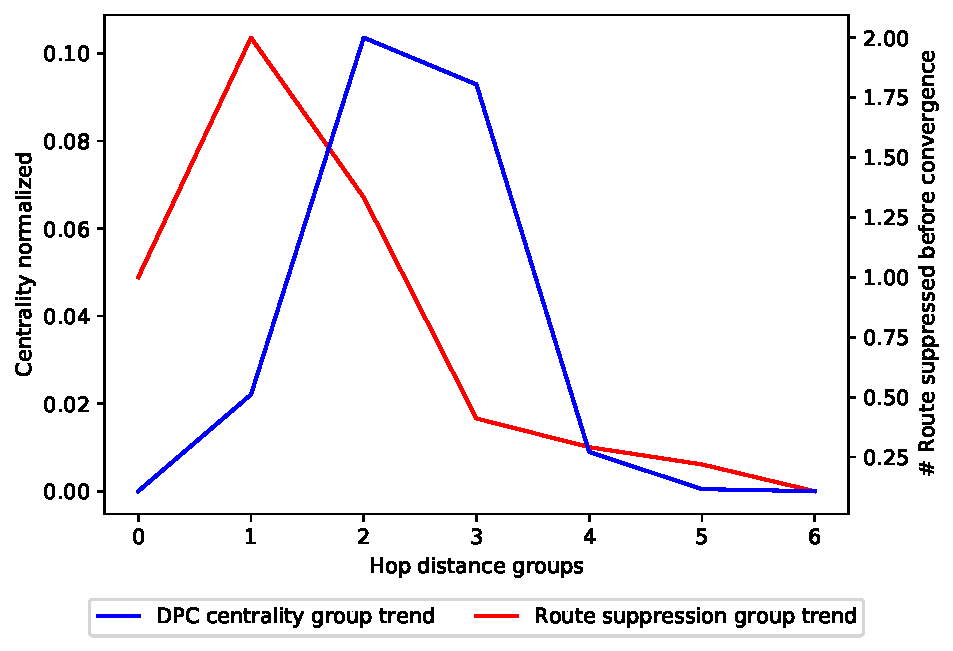
\includegraphics[width=\textwidth]{images/RFD/miceVSelephants/MultiMRAI/45/mice/cisco_1000_RFD_nodeConvergence_centVSsup_trend.pdf}
         \caption{RFD 2439 Strategy, \\MRAI=45s}
         \label{fig:1000_2439RFD_centVSsup_mices_MRAI45}
     \end{subfigure}
     \hfill
     \begin{subfigure}[b]{0.325\textwidth}
         \centering
         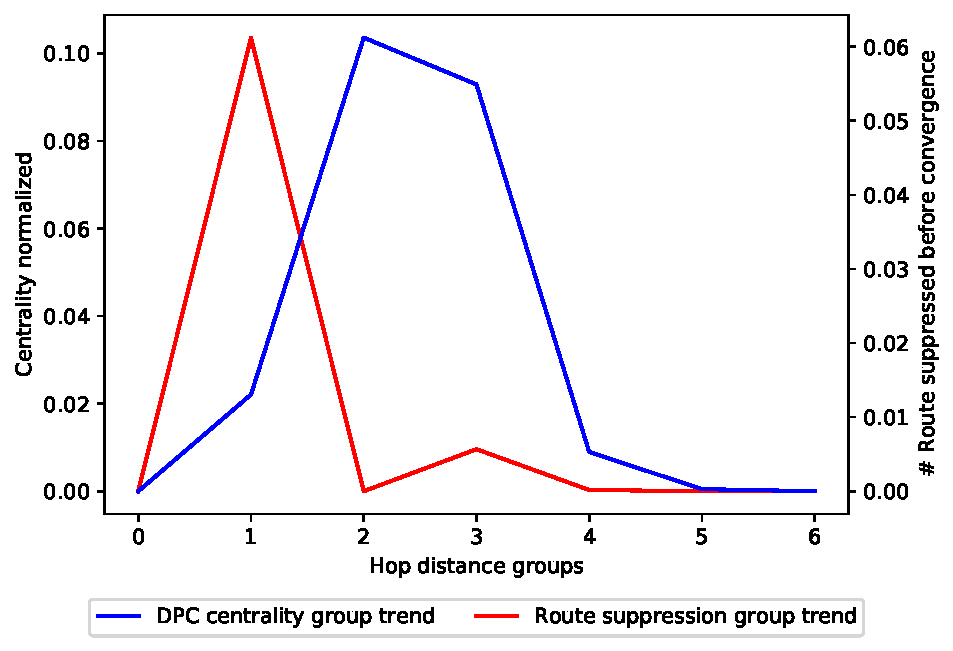
\includegraphics[width=\textwidth]{images/RFD/miceVSelephants/MultiMRAI/45/mice/cisco_1000_RFD_7196_aggressive_nodeConvergence_centVSsup_trend.pdf}
         \caption{RFD 7196 Aggressive Strategy, MRAI=45s}
         \label{fig:1000_7196RFDA_centVSsup_mices_MRAI45}
     \end{subfigure}
     \hfill
     \begin{subfigure}[b]{0.325\textwidth}
         \centering
         \includegraphics[width=\textwidth]{images/RFD/miceVSelephants/MultiMRAI/45/mice/cisco_1000_RFD_7196_conservative_nodeConvergence_centVSsup_trend.pdf}
         \caption{RFD 7196 Conservative Strategy, MRAI=45s}
         \label{fig:1000_7196RFDC_centVSsup_mices_MRAI45}
     \end{subfigure}
     \vfill
     \begin{subfigure}[b]{0.325\textwidth}
         \centering
         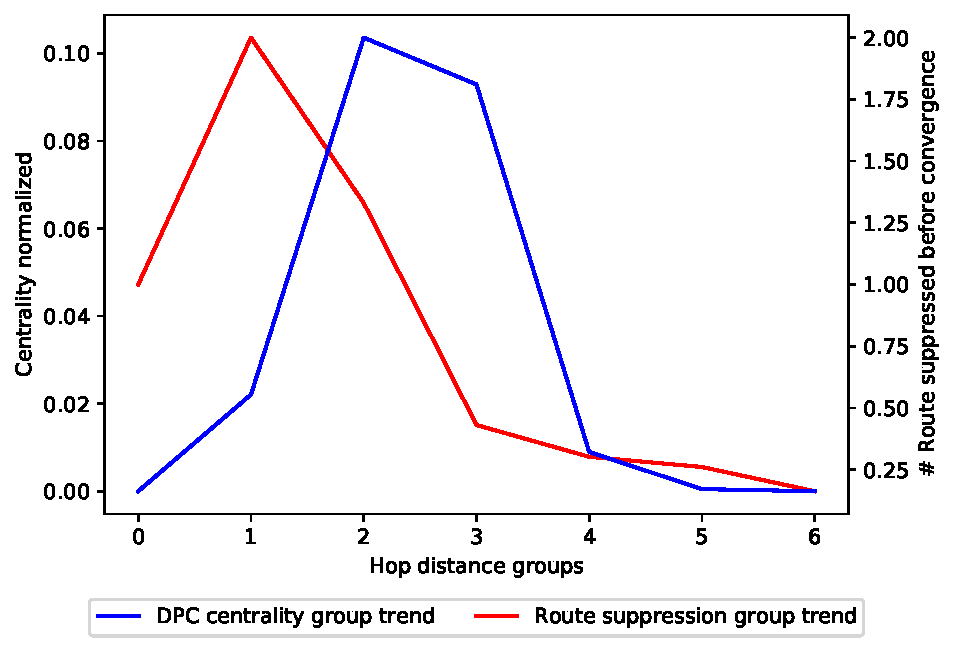
\includegraphics[width=\textwidth]{images/RFD/miceVSelephants/MultiMRAI/60/mice/cisco_1000_RFD_nodeConvergence_centVSsup_trend.pdf}
         \caption{RFD 2439 Strategy, \\MRAI=60s}
         \label{fig:1000_2439RFD_centVSsup_mices_MRAI60}
     \end{subfigure}
     \hfill
     \begin{subfigure}[b]{0.325\textwidth}
         \centering
         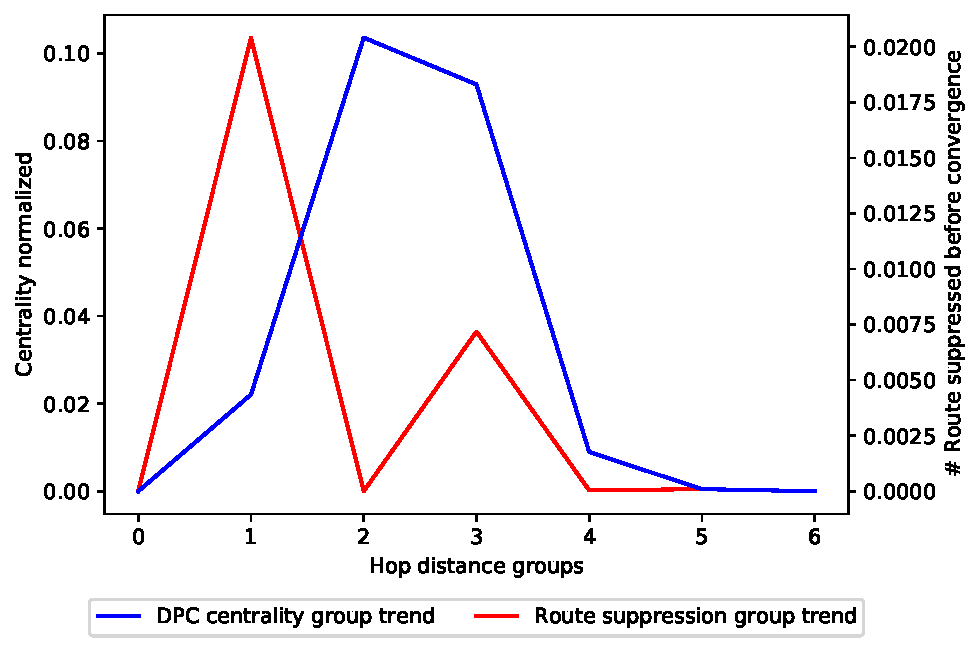
\includegraphics[width=\textwidth]{images/RFD/miceVSelephants/MultiMRAI/60/mice/cisco_1000_RFD_7196_aggressive_nodeConvergence_centVSsup_trend.pdf}
         \caption{RFD 7196 Aggressive Strategy, MRAI=60s}
         \label{fig:1000_7196RFDA_centVSsup_mices_MRAI60}
     \end{subfigure}
     \hfill
     \begin{subfigure}[b]{0.325\textwidth}
         \centering
         \includegraphics[width=\textwidth]{images/RFD/miceVSelephants/MultiMRAI/60/mice/cisco_1000_RFD_7196_conservative_nodeConvergence_centVSsup_trend.pdf}
         \caption{RFD 7196 Conservative Strategy, MRAI=60s}
         \label{fig:1000_7196RFDC_centVSsup_mices_MRAI60}
     \end{subfigure}
        \caption{Internet like topology 1000 nodes, random destination, 5 flaps, 300s delay, Suppression trend VS avg hop centrality}
        \label{fig:1000_RFD_centVSsup_mices}
\end{figure}

\begin{figure}[H]
     \centering
     \begin{subfigure}[b]{0.325\textwidth}
         \centering
         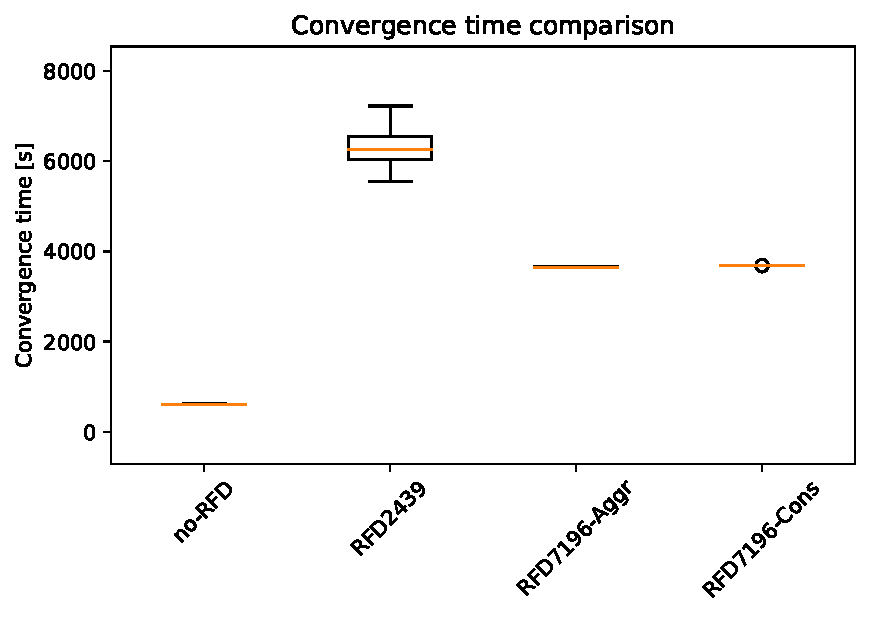
\includegraphics[width=\textwidth]{images/RFD/miceVSelephants/MultiMRAI/0/elephants/cisco_1000MRAI0_rfd_comparison_time_boxplot.pdf}
         \caption{Convergence time respect to the RFD strategy, MRAI=0s}
         \label{fig:1000_RFD_MRAI0_time_elephant}
     \end{subfigure}
     \hfill
     \begin{subfigure}[b]{0.325\textwidth}
         \centering
         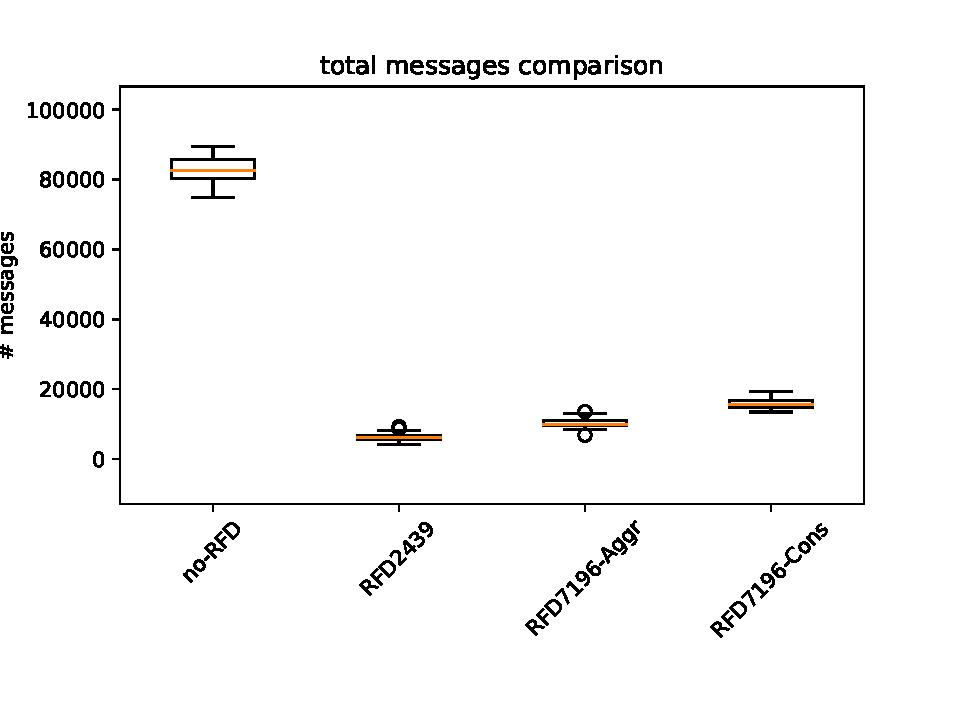
\includegraphics[width=\textwidth]{images/RFD/miceVSelephants/MultiMRAI/0/elephants/cisco_1000MRAI0_rfd_comparison_messages_boxplot.pdf}
         \caption{Number of messages respect to the RFD strategy, MRAI=0s}
         \label{fig:1000_RFD_MRAI0_messages_elephant}
     \end{subfigure}
     \hfill
     \begin{subfigure}[b]{0.325\textwidth}
         \centering
         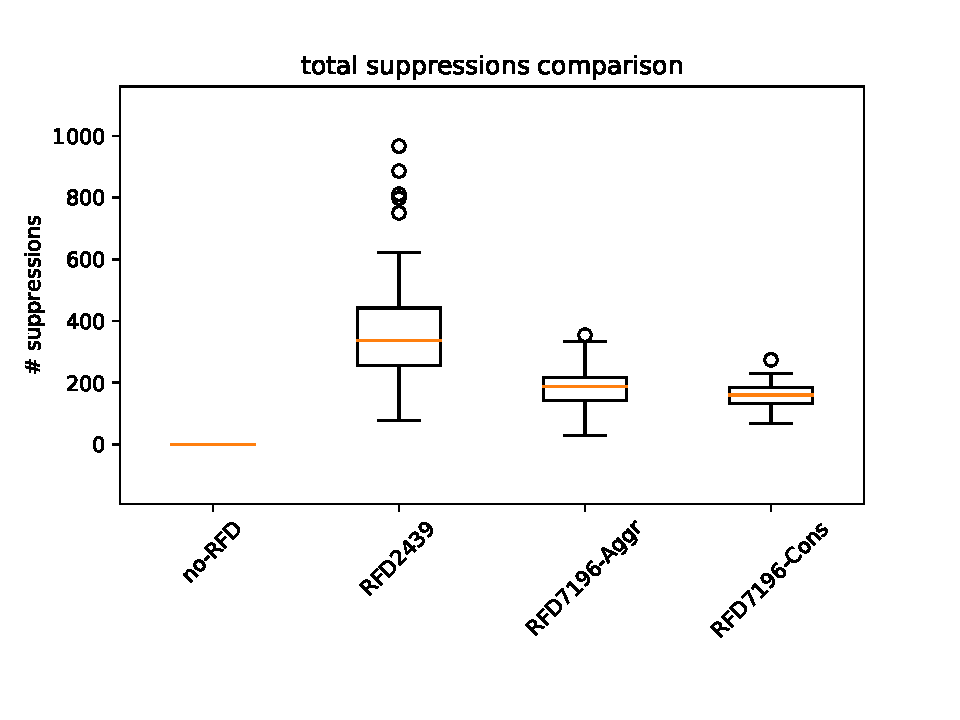
\includegraphics[width=\textwidth]{images/RFD/miceVSelephants/MultiMRAI/0/elephants/cisco_1000MRAI0_rfd_comparison_suppressions_boxplot.pdf}
         \caption{Number of suppressions respect to the RFD strategy, MRAI=0s}
         \label{fig:1000_RFD_MRAI0_suppressions_elephant}
     \end{subfigure}
     \vfill
     \begin{subfigure}[b]{0.325\textwidth}
         \centering
         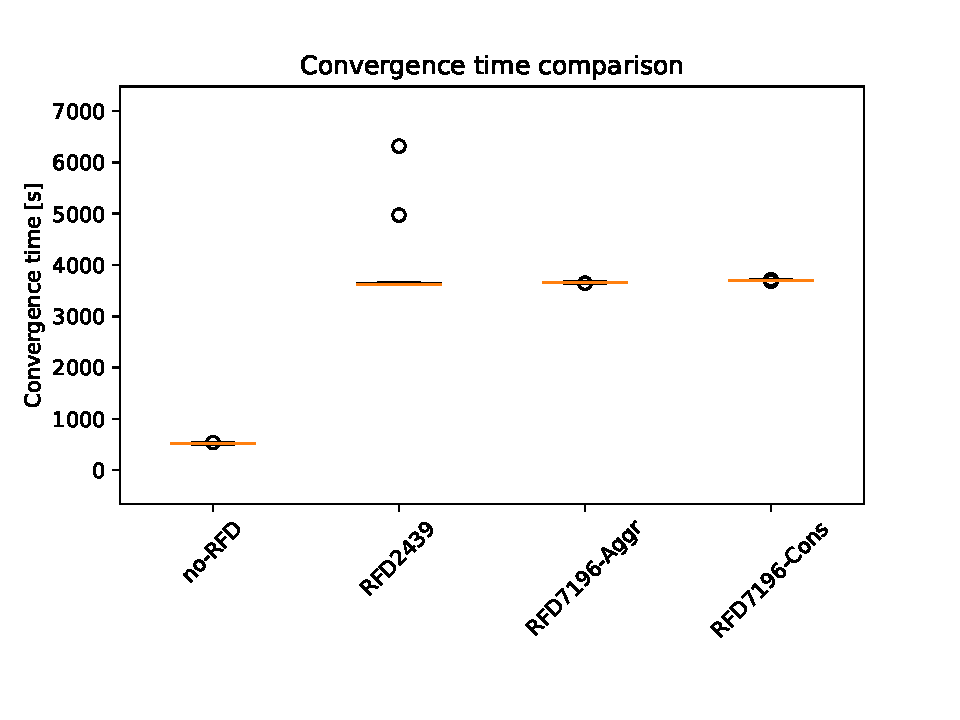
\includegraphics[width=\textwidth]{images/RFD/miceVSelephants/MultiMRAI/15/elephants/cisco_1000MRAI15_rfd_comparison_time_boxplot.pdf}
         \caption{Convergence time respect to the RFD strategy, MRAI=15s}
         \label{fig:1000_RFD_MRAI15_time_elephant}
     \end{subfigure}
     \hfill
     \begin{subfigure}[b]{0.325\textwidth}
         \centering
         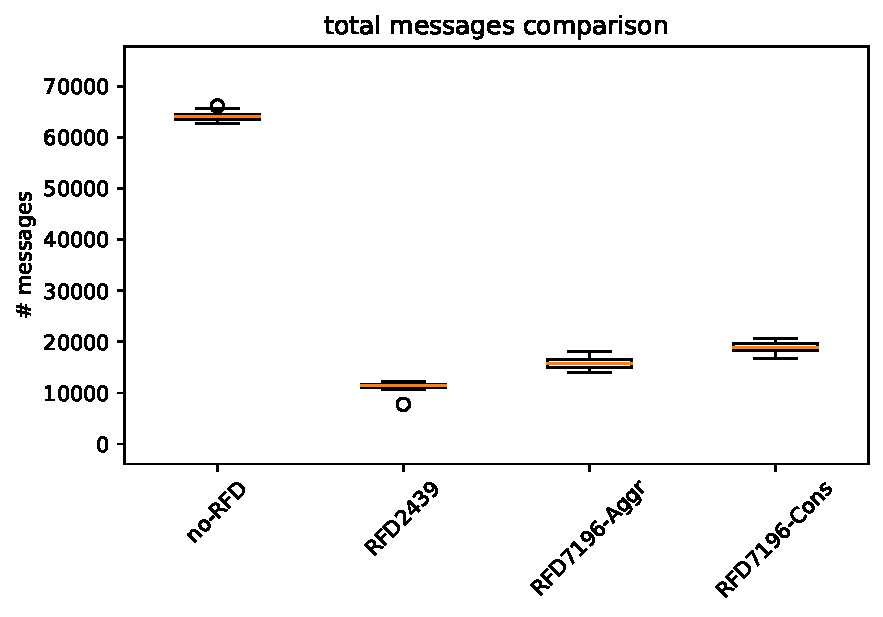
\includegraphics[width=\textwidth]{images/RFD/miceVSelephants/MultiMRAI/15/elephants/cisco_1000MRAI15_rfd_comparison_messages_boxplot.pdf}
         \caption{Number of messages respect to the RFD strategy, MRAI=15s}
         \label{fig:1000_RFD_MRAI15_messages_elephant}
     \end{subfigure}
     \hfill
     \begin{subfigure}[b]{0.325\textwidth}
         \centering
         \includegraphics[width=\textwidth]{images/RFD/miceVSelephants/MultiMRAI/15/elephants/cisco_1000MRAI15_rfd_comparison_suppressions_boxplot.pdf}
         \caption{Number of suppressions respect to the RFD strategy, MRAI=15s}
         \label{fig:1000_RFD_MRAI15_suppressions_elephant}
     \end{subfigure}
     \vfill
     \begin{subfigure}[b]{0.325\textwidth}
         \centering
         \includegraphics[width=\textwidth]{images/RFD/miceVSelephants/MultiMRAI/30/elephants/cisco_1000MRAI30_rfd_comparison_time_boxplot.pdf}
         \caption{Convergence time respect to the RFD strategy, MRAI=30s}
         \label{fig:1000_RFD_MRAI30_time_elephant}
     \end{subfigure}
     \hfill
     \begin{subfigure}[b]{0.325\textwidth}
         \centering
         \includegraphics[width=\textwidth]{images/RFD/miceVSelephants/MultiMRAI/30/elephants/cisco_1000MRAI30_rfd_comparison_messages_boxplot.pdf}
         \caption{Number of messages respect to the RFD strategy, MRAI=30s}
         \label{fig:1000_RFD_MRAI30_messages_elephant}
     \end{subfigure}
     \hfill
     \begin{subfigure}[b]{0.325\textwidth}
         \centering
         \includegraphics[width=\textwidth]{images/RFD/miceVSelephants/MultiMRAI/30/elephants/cisco_1000MRAI30_rfd_comparison_suppressions_boxplot.pdf}
         \caption{Number of suppressions respect to the RFD strategy, MRAI=30s}
         \label{fig:1000_RFD_MRAI30_suppressions_elephant}
     \end{subfigure}
     \vfill
     \begin{subfigure}[b]{0.325\textwidth}
         \centering
         \includegraphics[width=\textwidth]{images/RFD/miceVSelephants/MultiMRAI/45/elephants/cisco_1000MRAI45_rfd_comparison_time_boxplot.pdf}
         \caption{Convergence time respect to the RFD strategy, MRAI=45s}
         \label{fig:1000_RFD_MRAI45_time_elephant}
     \end{subfigure}
     \hfill
     \begin{subfigure}[b]{0.325\textwidth}
         \centering
         \includegraphics[width=\textwidth]{images/RFD/miceVSelephants/MultiMRAI/45/elephants/cisco_1000MRAI45_rfd_comparison_messages_boxplot.pdf}
         \caption{Number of messages respect to the RFD strategy, MRAI=30s}
         \label{fig:1000_RFD_MRAI45_messages_elephant}
     \end{subfigure}
     \hfill
     \begin{subfigure}[b]{0.325\textwidth}
         \centering
         \includegraphics[width=\textwidth]{images/RFD/miceVSelephants/MultiMRAI/45/elephants/cisco_1000MRAI45_rfd_comparison_suppressions_boxplot.pdf}
         \caption{Number of suppressions respect to the RFD strategy, MRAI=45s}
         \label{fig:1000_RFD_MRAI45_suppressions_elephant}
     \end{subfigure}
     \vfill
     \begin{subfigure}[b]{0.325\textwidth}
         \centering
         \includegraphics[width=\textwidth]{images/RFD/miceVSelephants/MultiMRAI/60/elephants/cisco_1000MRAI60_rfd_comparison_time_boxplot.pdf}
         \caption{Convergence time respect to the RFD strategy, MRAI=60s}
         \label{fig:1000_RFD_MRAI60_time_elephant}
     \end{subfigure}
     \hfill
     \begin{subfigure}[b]{0.325\textwidth}
         \centering
         \includegraphics[width=\textwidth]{images/RFD/miceVSelephants/MultiMRAI/60/elephants/cisco_1000MRAI60_rfd_comparison_messages_boxplot.pdf}
         \caption{Number of messages respect to the RFD strategy, MRAI=60s}
         \label{fig:1000_RFD_MRAI60_messages_elephant}
     \end{subfigure}
     \hfill
     \begin{subfigure}[b]{0.325\textwidth}
         \centering
         \includegraphics[width=\textwidth]{images/RFD/miceVSelephants/MultiMRAI/60/elephants/cisco_1000MRAI60_rfd_comparison_suppressions_boxplot.pdf}
         \caption{Number of suppressions respect to the RFD strategy, MRAI=60s}
         \label{fig:1000_RFD_MRAI60_suppressions_elephant}
     \end{subfigure}
        \caption{Internet like topology 1000 nodes, random destination, 100 flaps, 3s delay, Network performances}
        \label{fig:1000_RFD_MRAI30_elephant}
\end{figure}

\begin{figure}[H]
     \centering
     \begin{subfigure}[b]{0.325\textwidth}
         \centering
         \includegraphics[width=\textwidth]{images/RFD/miceVSelephants/MultiMRAI/0/elephants/cisco_1000_RFD_nodeConvergence_centVSsup_trend.pdf}
         \caption{RFD 2439 Strategy, \\MRAI=0s}
         \label{fig:1000_2439RFD_centVSsup_elephants_MRAI0}
     \end{subfigure}
     \hfill
     \begin{subfigure}[b]{0.325\textwidth}
         \centering
         \includegraphics[width=\textwidth]{images/RFD/miceVSelephants/MultiMRAI/0/elephants/cisco_1000_RFD_7196_aggressive_nodeConvergence_centVSsup_trend.pdf}
         \caption{RFD 7196 Aggressive Strategy, MRAI=0s}
         \label{fig:1000_7196RFDA_centVSsup_elephants_MRAI0}
     \end{subfigure}
     \hfill
     \begin{subfigure}[b]{0.325\textwidth}
         \centering
         \includegraphics[width=\textwidth]{images/RFD/miceVSelephants/MultiMRAI/0/elephants/cisco_1000_RFD_7196_conservative_nodeConvergence_centVSsup_trend.pdf}
         \caption{RFD 7196 Conservative Strategy, MRAI=0s}
         \label{fig:1000_7196RFDC_centVSsup_elephants_MRAI0}
     \end{subfigure}
     \vfill
     \begin{subfigure}[b]{0.325\textwidth}
         \centering
         \includegraphics[width=\textwidth]{images/RFD/miceVSelephants/MultiMRAI/15/elephants/cisco_1000_RFD_nodeConvergence_centVSsup_trend.pdf}
         \caption{RFD 2439 Strategy, \\MRAI=15s}
         \label{fig:1000_2439RFD_centVSsup_elephants_MRAI15}
     \end{subfigure}
     \hfill
     \begin{subfigure}[b]{0.325\textwidth}
         \centering
         \includegraphics[width=\textwidth]{images/RFD/miceVSelephants/MultiMRAI/15/elephants/cisco_1000_RFD_7196_aggressive_nodeConvergence_centVSsup_trend.pdf}
         \caption{RFD 7196 Aggressive Strategy, MRAI=15s}
         \label{fig:1000_7196RFDA_centVSsup_elephants_MRAI15}
     \end{subfigure}
     \hfill
     \begin{subfigure}[b]{0.325\textwidth}
         \centering
         \includegraphics[width=\textwidth]{images/RFD/miceVSelephants/MultiMRAI/15/elephants/cisco_1000_RFD_7196_conservative_nodeConvergence_centVSsup_trend.pdf}
         \caption{RFD 7196 Conservative Strategy, MRAI=15s}
         \label{fig:1000_7196RFDC_centVSsup_elephants_MRAI15}
     \end{subfigure}
     \vfill
     \begin{subfigure}[b]{0.325\textwidth}
         \centering
         \includegraphics[width=\textwidth]{images/RFD/miceVSelephants/MultiMRAI/30/elephants/cisco_1000_RFD_nodeConvergence_centVSsup_trend.pdf}
         \caption{RFD 2439 Strategy, \\MRAI=30s}
         \label{fig:1000_2439RFD_centVSsup_elephants_MRAI30}
     \end{subfigure}
     \hfill
     \begin{subfigure}[b]{0.325\textwidth}
         \centering
         \includegraphics[width=\textwidth]{images/RFD/miceVSelephants/MultiMRAI/30/elephants/cisco_1000_RFD_7196_aggressive_nodeConvergence_centVSsup_trend.pdf}
         \caption{RFD 7196 Aggressive Strategy, MRAI=30s}
         \label{fig:1000_7196RFDA_centVSsup_elephants_MRAI30}
     \end{subfigure}
     \hfill
     \begin{subfigure}[b]{0.325\textwidth}
         \centering
         \includegraphics[width=\textwidth]{images/RFD/miceVSelephants/MultiMRAI/30/elephants/cisco_1000_RFD_7196_conservative_nodeConvergence_centVSsup_trend.pdf}
         \caption{RFD 7196 Conservative Strategy, MRAI=30s}
         \label{fig:1000_7196RFDC_centVSsup_elephants_MRAI30}
     \end{subfigure}
     \vfill
     \begin{subfigure}[b]{0.325\textwidth}
         \centering
         \includegraphics[width=\textwidth]{images/RFD/miceVSelephants/MultiMRAI/45/elephants/cisco_1000_RFD_nodeConvergence_centVSsup_trend.pdf}
         \caption{RFD 2439 Strategy, \\MRAI=45s}
         \label{fig:1000_2439RFD_centVSsup_elephants_MRAI45}
     \end{subfigure}
     \hfill
     \begin{subfigure}[b]{0.325\textwidth}
         \centering
         \includegraphics[width=\textwidth]{images/RFD/miceVSelephants/MultiMRAI/45/elephants/cisco_1000_RFD_7196_aggressive_nodeConvergence_centVSsup_trend.pdf}
         \caption{RFD 7196 Aggressive Strategy, MRAI=45s}
         \label{fig:1000_7196RFDA_centVSsup_elephants_MRAI45}
     \end{subfigure}
     \hfill
     \begin{subfigure}[b]{0.325\textwidth}
         \centering
         \includegraphics[width=\textwidth]{images/RFD/miceVSelephants/MultiMRAI/45/elephants/cisco_1000_RFD_7196_conservative_nodeConvergence_centVSsup_trend.pdf}
         \caption{RFD 7196 Conservative Strategy, MRAI=45s}
         \label{fig:1000_7196RFDC_centVSsup_elephants_MRAI45}
     \end{subfigure}
     \vfill
     \begin{subfigure}[b]{0.325\textwidth}
         \centering
         \includegraphics[width=\textwidth]{images/RFD/miceVSelephants/MultiMRAI/60/elephants/cisco_1000_RFD_nodeConvergence_centVSsup_trend.pdf}
         \caption{RFD 2439 Strategy, \\MRAI=60s}
         \label{fig:1000_2439RFD_centVSsup_elephants_MRAI60}
     \end{subfigure}
     \hfill
     \begin{subfigure}[b]{0.325\textwidth}
         \centering
         \includegraphics[width=\textwidth]{images/RFD/miceVSelephants/MultiMRAI/60/elephants/cisco_1000_RFD_7196_aggressive_nodeConvergence_centVSsup_trend.pdf}
         \caption{RFD 7196 Aggressive Strategy, MRAI=60s}
         \label{fig:1000_7196RFDA_centVSsup_elephants_MRAI60}
     \end{subfigure}
     \hfill
     \begin{subfigure}[b]{0.325\textwidth}
         \centering
         \includegraphics[width=\textwidth]{images/RFD/miceVSelephants/MultiMRAI/60/elephants/cisco_1000_RFD_7196_conservative_nodeConvergence_centVSsup_trend.pdf}
         \caption{RFD 7196 Conservative Strategy, MRAI=60s}
         \label{fig:1000_7196RFDC_centVSsup_elephants_MRAI60}
     \end{subfigure}
        \caption{Internet like topology 1000 nodes, random destination, 100 flaps, 3s delay, Suppression trend VS avg hop centrality}
        \label{fig:1000_RFD_centVSsup_elephants}
\end{figure}


\end{document}
